%=====================================================================
% Informe Final — Análisis Exploratorio de Datos
% Curso: Tópicos en Ciencia de Datos / Ciencia de Datos y Big Data (UNSA)
% Compilar con: pdflatex -> bibtex (opcional) -> pdflatex x2
%=====================================================================
\documentclass[11pt,a4paper]{article}

\usepackage[utf8]{inputenc}
\usepackage[T1]{fontenc}
\usepackage[spanish,es-tabla]{babel}
\usepackage[margin=2.5cm]{geometry}
\usepackage{graphicx}
\usepackage{booktabs}
\usepackage{longtable}
\usepackage{array}
\usepackage{amsmath,amssymb}
\usepackage{float}
\usepackage{caption}
\usepackage{subcaption}
\usepackage{xcolor}
\usepackage{enumitem}
\usepackage{listings}
\usepackage[hidelinks]{hyperref}
\usepackage{tikz}
\usetikzlibrary{arrows.meta,positioning,shapes.geometric,fit,backgrounds}

\graphicspath{{figures/}}

\definecolor{azulunsa}{RGB}{20,70,120}
\definecolor{grisclaro}{RGB}{240,240,240}

\captionsetup{font=small,labelfont=bf}
\setlength{\parskip}{0.4em}

\lstset{
  basicstyle=\ttfamily\footnotesize,
  backgroundcolor=\color{grisclaro},
  breaklines=true,
  frame=single,
  numbers=left,
  numberstyle=\tiny,
  language=Python
}

%--------------------------------------------------------------------
\begin{document}

%=====================  PORTADA  =====================================
\begin{titlepage}
\centering
\vspace*{1.5cm}

{\large\scshape Universidad Nacional de San Agustín de Arequipa}\\[0.3cm]
{\large Escuela Profesional de Ciencia de la Computación}\\[0.2cm]
{\large Curso: Tópicos en Ciencia de Datos}\\[1.5cm]

\rule{\textwidth}{1.2pt}\\[0.5cm]
{\Huge\bfseries Informe Final:\\[0.3cm] Análisis Exploratorio de Datos}\\[0.5cm]
{\Large\itshape Exploración visual de datasets de imágenes mediante\\ clustering jerárquico y características visuales cuantificables}\\[0.4cm]
\rule{\textwidth}{1.2pt}\\[2cm]

{\large\textbf{Estudiante}}\\[0.3cm]
{\large Diego Raúl Rivas Huanca}\\
{\large Guerra Chura Joan Leonard}\\[2cm]

{\large\textbf{Docente}}\\[0.3cm]
{\large Ana María Cuadros Valdivia}\\[2cm]

{\large Fecha de presentación: 19 de septiembre de 2026}\\[1cm]
{\large Arequipa -- Perú}

\vfill
\end{titlepage}

\tableofcontents
\newpage

%=====================  1. PROBLEMA  =================================
\section{Definición del problema}

\subsection*{¿Cuál es el problema que se quiere abordar?}

Los grandes conjuntos de datos de imágenes utilizados en aprendizaje automático
(CIFAR-10, CIFAR-100, ImageNet) carecen de atributos estructurados. A diferencia
de un dataset tabular, donde cada registro posee columnas sobre las cuales se
puede filtrar, agrupar y ordenar, una imagen solo trae consigo su etiqueta de
clase. Esta ausencia de atributos convierte a la exploración de estos datasets en
una tarea difícil: no es posible responder con facilidad preguntas como
\emph{¿qué tipos de imágenes contiene realmente esta clase?},
\emph{¿por qué estas imágenes quedan agrupadas juntas?} o
\emph{¿qué subgrupos del dataset son problemáticos?}

El sistema \textsc{DendroMap} \cite{bertucci2023} aborda parcialmente este
problema: extrae representaciones de alta dimensión (\emph{embeddings}) desde una
red ResNet50, aplica \emph{clustering} jerárquico aglomerativo y representa el
dendrograma resultante mediante un \emph{treemap} interactivo con
\emph{zoom} semántico. Con ello, el usuario puede pasar de una visión general
del dataset al detalle de un subgrupo. Sin embargo, la estructura que
\textsc{DendroMap} muestra es opaca en cuanto a su causa: el sistema revela
\textbf{dónde} están los grupos, pero no ofrece atributos interpretables que
expliquen \textbf{por qué} esos grupos se formaron. Los propios autores señalan,
en su sección de trabajo futuro, que usar atributos interpretables para la
construcción de los árboles es una línea prometedora aún no explorada.

Por lo tanto, el problema que se aborda en este trabajo es:

\begin{quote}
\itshape
La estructura de agrupamiento que emerge de las representaciones profundas de un
dataset de imágenes no es interpretable por sí sola. No se dispone de atributos
cuantificables que permitan caracterizar los clusters, explicar por qué imágenes
de clases distintas se agrupan juntas, o por qué una misma clase se fragmenta en
subgrupos visualmente heterogéneos.
\end{quote}

\subsection*{¿Por qué es importante resolverlo?}

\begin{itemize}[leftmargin=*]
  \item \textbf{Relevancia científica y de ingeniería de datos.} La corriente de
  \emph{Data-Centric AI} sostiene que la calidad del dataset determina en mayor
  medida el desempeño del modelo que la arquitectura elegida. Entender la
  composición interna de un dataset es un prerrequisito para decidir qué datos
  recolectar, cómo etiquetar y cómo mitigar sesgos.
  \item \textbf{Relevancia social.} Los sesgos visuales sistemáticos (tonos de
  piel, iluminación, fondos predominantes) se propagan a los modelos entrenados.
  Disponer de atributos cuantificables permite auditarlos de forma objetiva y no
  solo mediante inspección visual subjetiva.
  \item \textbf{Relevancia práctica.} Identificar subgrupos de baja calidad
  visual (bajo contraste, alta compresión, objeto pequeño) permite priorizar el
  esfuerzo de re-etiquetado o de recolección de datos adicionales.
\end{itemize}

\subsection*{¿Qué área del conocimiento involucra?}

El trabajo se ubica en la intersección de \textbf{Visual Analytics} e
\textbf{Interacción Humano-Computador} (visualización de información,
\emph{treemaps}, vistas coordinadas), \textbf{Visión Computacional}
(representaciones profundas, descriptores de bajo nivel) y \textbf{Ciencia de
Datos} (análisis exploratorio, clustering, estadística descriptiva).

\subsection*{¿Qué se espera lograr al final del proyecto?}

Al final del proyecto de Visual Analytics se espera disponer de una herramienta
web interactiva (D3.js) que permita explorar un dataset de imágenes combinando
la estructura jerárquica de \textsc{DendroMap} con un panel de características
visuales cuantificables, de modo que el analista pueda responder, para cualquier
cluster seleccionado, la pregunta \emph{¿qué distingue visualmente a este grupo
del resto del dataset?} El presente informe exploratorio constituye la etapa
previa: establecer qué características son informativas, qué problemas de
calidad existen y qué comportamientos merecen ser explorados de forma
interactiva.

%=====================  2. HIPÓTESIS  ================================
\section{Hipótesis y preguntas de investigación}

\subsection{Motivación}

Las hipótesis surgen de tres fuentes:

\begin{enumerate}[leftmargin=*]
  \item \textbf{Del artículo científico base.} \textsc{DendroMap} \cite{bertucci2023}
  reporta como hallazgos principales la diversidad de imágenes, los subgrupos con
  bajo desempeño y los errores de clasificación. Explícitamente deja abierta la
  construcción de árboles a partir de atributos interpretables. Nuestras hipótesis
  se sitúan en ese vacío: no repetimos sus hallazgos, los complementamos.
  \item \textbf{Del conocimiento del dominio.} En visión computacional es conocido
  que las primeras capas de una CNN responden a bordes, color y textura. Es
  razonable suponer que parte de la estructura de los \emph{embeddings} profundos
  siga correlacionada con descriptores de bajo nivel calculables directamente
  sobre los píxeles.
  \item \textbf{De un cruce con datos externos.} El dataset CIFAR-10H
  \cite{peterson2019} aporta anotaciones humanas múltiples (aprox.\ 50 por imagen)
  sobre el conjunto de prueba de CIFAR-10. Esto permite medir la
  \emph{ambigüedad percibida por humanos} de cada imagen y contrastarla contra sus
  características visuales, algo que \textsc{DendroMap} no analiza.
\end{enumerate}

\subsection{Hipótesis formuladas como preguntas}

\begin{description}[leftmargin=0pt,style=nextline]
  \item[Hipótesis 1 : Confluencia visual entre clases]
  ¿Existen clusters del dendrograma que agrupan imágenes de clases semánticamente
  distintas, y ese agrupamiento es explicable mediante características visuales
  cuantificables (brillo, contraste, saturación, entropía, densidad de bordes,
  color dominante)?

  \item[Hipótesis 2 : Divergencia visual dentro de una clase]
  ¿Una misma clase de CIFAR-10 se fragmenta en subgrupos visualmente diferenciados,
  de modo que la etiqueta semántica oculta más de un patrón visual? Si es así,
  ¿qué características separan a esos subgrupos con mayor poder discriminante?

  \item[Hipótesis 3 : Ambigüedad humana y calidad visual]
  ¿Las imágenes con mayor desacuerdo entre anotadores humanos (entropía de la
  distribución de votos en CIFAR-10H) se concentran en clusters específicos y
  presentan un perfil de características visuales distinto (menor contraste,
  mayor entropía de imagen, objeto de menor tamaño aparente) respecto de las
  imágenes de consenso unánime?
\end{description}

Las tres preguntas son específicas, respondibles con los datos disponibles y
están directamente conectadas con el problema definido en la Sección~1: todas
apuntan a dotar de atributos interpretables a la estructura de agrupamiento.

%=====================  3. PLAN DE ANÁLISIS  =========================
\section{Plan de análisis}

\subsection{Ciclo de vida de Ciencia de Datos aplicado al proyecto}

El trabajo sigue las etapas del ciclo de vida de Ciencia de Datos. La
Figura~\ref{fig:ciclovida} resume el recorrido y la Tabla~\ref{tab:ciclovida} lo
instancia para este proyecto.

\begin{figure}[H]
\centering
\begin{tikzpicture}[
  etapa/.style={draw,rounded corners=3pt,fill=azulunsa!12,minimum height=1.0cm,
                text width=2.7cm,align=center,font=\footnotesize},
  ar/.style={-{Latex[length=2.2mm]},thick},
  arv/.style={-{Latex[length=2.2mm]},thick,dashed,gray}
]
\node[etapa] (p1) at (0,0)      {Formulación\\de preguntas};
\node[etapa] (p2) at (3.6,0)    {Adquisición\\de datos};
\node[etapa] (p3) at (7.2,0)    {Wrangling\\y limpieza};
\node[etapa] (p4) at (10.8,0)   {Análisis\\exploratorio};
\node[etapa] (p5) at (7.2,-2.2) {Modelos\\auxiliares};
\node[etapa] (p6) at (3.6,-2.2) {Comunicación\\y decisión};

\draw[ar] (p1) -- (p2);
\draw[ar] (p2) -- (p3);
\draw[ar] (p3) -- (p4);
\draw[ar] (p4) -- (p5);
\draw[ar] (p5) -- (p6);
\draw[arv] (p4.north) -- ++(0,0.6) -| node[above,pos=0.25,font=\scriptsize]
  {refinamiento de las hipótesis} (p1.north);
\draw[arv] (p5.north) -- (p4.south);
\end{tikzpicture}
\caption{Ciclo de vida de Ciencia de Datos instanciado para la exploración de
datasets de imágenes. Las flechas punteadas indican que la formulación de
preguntas se refina tras la exploración.}
\label{fig:ciclovida}
\end{figure}

\begin{table}[H]
\centering
\small
\begin{tabular}{@{}p{3.2cm}p{11cm}@{}}
\toprule
\textbf{Etapa} & \textbf{Instanciación en este proyecto} \\
\midrule
Formulación de preguntas & Tres hipótesis derivadas de \textsc{DendroMap}, del dominio y del cruce con CIFAR-10H (Sección~2). \\
Adquisición de datos & Descarga de CIFAR-10 y CIFAR-100 desde el sitio oficial de la Universidad de Toronto; descarga de CIFAR-10H desde su repositorio público. \\
Comprensión y \emph{wrangling} & Deserialización de los \emph{batches} \texttt{pickle}, reconstrucción de los tensores $32{\times}32{\times}3$, unión de metadatos y verificación de integridad. \\
Limpieza & Detección de duplicados exactos y casi-duplicados, imágenes degeneradas (varianza nula), valores atípicos en las características derivadas. \\
Análisis exploratorio (AED) & Estadística descriptiva, distribuciones, correlaciones Pearson/Spearman, visualizaciones por clase y por cluster. \\
Construcción de modelos auxiliares & Extracción de \emph{embeddings} con ResNet50 y \emph{clustering} jerárquico aglomerativo (Ward, distancia euclidiana), reproduciendo el procedimiento de \textsc{DendroMap}. \\
Comunicación y decisión & Este informe y la definición de los requisitos de la herramienta de Visual Analytics. \\
\bottomrule
\end{tabular}
\caption{Etapas del ciclo de vida y su instanciación.}
\label{tab:ciclovida}
\end{table}

\subsection{Pipeline de datos}

El \emph{pipeline} implementado es lineal con un punto de bifurcación: las
imágenes alimentan simultáneamente el extractor de características de bajo nivel
y el extractor de \emph{embeddings} profundos. Ambos caminos convergen en una
tabla única en la que cada fila es una imagen.

\begin{figure}[H]
\centering
\begin{tikzpicture}[
  node distance=0.55cm and 0.9cm,
  box/.style={draw,rounded corners=2pt,fill=grisclaro,minimum height=0.85cm,
              text width=2.55cm,align=center,font=\footnotesize},
  dato/.style={draw,rounded corners=2pt,fill=azulunsa!15,minimum height=0.85cm,
              text width=2.55cm,align=center,font=\footnotesize},
  ar/.style={-{Latex[length=2mm]},thick}
]
\node[dato] (raw) {CIFAR-10/100\\\texttt{data\_batch\_*}};
\node[box,right=of raw] (wr) {Wrangling\\deserializar,\\reconstruir RGB};
\node[box,above right=0.1cm and 0.9cm of wr] (feat) {Características\\de bajo nivel\\(OpenCV/NumPy)};
\node[box,below right=0.1cm and 0.9cm of wr] (emb) {Embeddings\\ResNet50\\(512/1024-D)};
\node[box,below=of emb] (clu) {Clustering\\jerárquico\\(Ward)};
\node[dato,right=2.6cm of wr] (tab) {Tabla unificada\\1 fila = 1 imagen};
\node[box,right=of tab] (eda) {AED\\estadística +\\visualización};
\node[dato,right=of eda] (out) {Hallazgos\\$\rightarrow$ requisitos\\Visual Analytics};
\node[dato,below=of raw] (h10) {CIFAR-10H\\votos humanos};

\draw[ar] (raw) -- (wr);
\draw[ar] (wr) -- (feat);
\draw[ar] (wr) -- (emb);
\draw[ar] (emb) -- (clu);
\draw[ar] (feat) -- (tab);
\draw[ar] (clu.east) -- ++(0.3,0) |- (tab);
\draw[ar] (h10.east) -| (tab);
\draw[ar] (tab) -- (eda);
\draw[ar] (eda) -- (out);
\end{tikzpicture}
\caption{Pipeline de datos del proyecto. El cruce con datos externos (CIFAR-10H)
se incorpora a nivel de registro mediante el índice de la imagen en el conjunto
de prueba.}
\label{fig:pipeline}
\end{figure}

La tabla unificada resultante tiene el siguiente esquema conceptual:

\begin{center}
\small
\begin{tabular}{@{}lll@{}}
\toprule
\textbf{Bloque} & \textbf{Origen} & \textbf{Ejemplo de columnas} \\
\midrule
Identificación & Dataset original & \texttt{img\_id}, \texttt{split}, \texttt{clase}, \texttt{superclase} \\
Características visuales & Calculadas & \texttt{brillo}, \texttt{contraste}, \texttt{saturacion}, \texttt{entropia}, \texttt{bordes} \\
Estructura & Embeddings + clustering & \texttt{cluster\_k8}, \texttt{cluster\_k18}, \texttt{profundidad} \\
Datos externos & CIFAR-10H & \texttt{n\_votos}, \texttt{entropia\_humana}, \texttt{consenso} \\
\bottomrule
\end{tabular}
\end{center}

%=====================  4. FUENTE DE DATOS  ==========================
\section{Fuente de datos}

\subsection{Origen}

\begin{itemize}[leftmargin=*]
  \item \textbf{CIFAR-10 y CIFAR-100.} Recolectados por Alex Krizhevsky, Vinod
  Nair y Geoffrey Hinton en la Universidad de Toronto \cite{krizhevsky2009}.
  Constituyen subconjuntos etiquetados del dataset \emph{80 Million Tiny Images},
  recopilado mediante consultas a buscadores web. Las etiquetas fueron asignadas
  por anotadores humanos pagados, con un protocolo que exigía que el objeto de la
  clase fuera prominente en la imagen. Disponibles públicamente en
  \url{https://www.cs.toronto.edu/~kriz/cifar.html}.
  \item \textbf{CIFAR-10H.} Publicado por Peterson et al.\ \cite{peterson2019},
  contiene aproximadamente 500\,000 anotaciones humanas recolectadas sobre las
  10\,000 imágenes del conjunto de prueba de CIFAR-10 (alrededor de 50 anotadores
  por imagen). Se utiliza aquí como fuente externa para medir ambigüedad
  perceptual.
\end{itemize}

\subsection{Área del conocimiento}

Visión computacional y aprendizaje automático supervisado. CIFAR es uno de los
\emph{benchmarks} más utilizados para clasificación de imágenes, y es
precisamente el dataset empleado por \textsc{DendroMap} en su estudio de usuarios
y en sus experimentos de preservación de distancias.

\subsection{Problema que se quiere resolver con estos datos}

A nivel computacional, el problema original de CIFAR es la clasificación
multiclase de imágenes de baja resolución. En nuestro trabajo el dataset se
reutiliza con otro fin: no entrenamos un clasificador, sino que usamos el dataset
como objeto de estudio en sí mismo, para caracterizar su estructura interna.

\subsection{Por qué se capturaron las variables y su importancia}

Las variables originales son mínimas: el tensor de píxeles y la etiqueta de
clase. Esa pobreza de atributos es, precisamente, el problema que motiva el
trabajo. Las variables derivadas que construimos responden a criterios
perceptuales bien establecidos en procesamiento de imágenes:

\begin{itemize}[leftmargin=*]
  \item \textbf{Brillo y contraste}: condiciones de captura e iluminación.
  \item \textbf{Saturación y color dominante}: paleta cromática del objeto y del fondo.
  \item \textbf{Entropía}: complejidad informacional, proxy de la riqueza de textura.
  \item \textbf{Densidad de bordes}: cantidad de estructura y detalle.
  \item \textbf{Uniformidad del fondo}: desviación estándar de la banda perimetral.
\end{itemize}

\subsection{Referencias de los papers base}

Los artículos base del conjunto de datos y del método son
\cite{krizhevsky2009} (dataset), \cite{bertucci2023} (método de exploración
visual) y \cite{peterson2019} (anotaciones humanas). Las referencias completas
figuran en la Sección~\ref{sec:refs}.

%=====================  5. FORMATO ORIGINAL  =========================
\section{Formato original del dataset}

CIFAR-10 se distribuye como un archivo \texttt{cifar-10-python.tar.gz} que, al
descomprimirse, contiene seis archivos serializados con el módulo \texttt{pickle}
de Python: \texttt{data\_batch\_1} a \texttt{data\_batch\_5} (10\,000 imágenes
cada uno) y \texttt{test\_batch}. Cada archivo es un diccionario con las claves
\texttt{data}, \texttt{labels}, \texttt{filenames} y \texttt{batch\_label}.
Existe además \texttt{batches.meta}, con los nombres legibles de las clases.

Particularidades de lectura que deben documentarse:

\begin{enumerate}[leftmargin=*]
  \item Los archivos fueron serializados con Python 2, por lo que deben leerse con
  \texttt{pickle.load(f, encoding='bytes')} y las claves resultan ser
  \emph{bytes} (\texttt{b'data'}) y no cadenas.
  \item \texttt{data} es un arreglo \texttt{uint8} de forma $10000 \times 3072$.
  Los 3072 valores se ordenan por canal: los primeros 1024 corresponden al canal
  rojo, los siguientes 1024 al verde y los últimos 1024 al azul; dentro de cada
  bloque el orden es por filas. La reconstrucción correcta requiere
  \texttt{reshape(-1, 3, 32, 32).transpose(0, 2, 3, 1)}. Omitir la transposición
  produce imágenes irreconocibles sin que se emita ningún error.
  \item No hay encabezados, tipos declarados ni valores faltantes en el sentido
  tabular: los datos son un tensor denso.
  \item CIFAR-100 sigue el mismo formato, pero con las claves
  \texttt{fine\_labels} (100 clases) y \texttt{coarse\_labels} (20 superclases).
  \item CIFAR-10H se distribuye como un CSV de anotaciones individuales, cuyo
  orden de filas \emph{no} coincide con el orden del \texttt{test\_batch}: la
  unión debe hacerse por la columna de índice de imagen provista en el CSV.
\end{enumerate}

\begin{figure}[H]
\centering
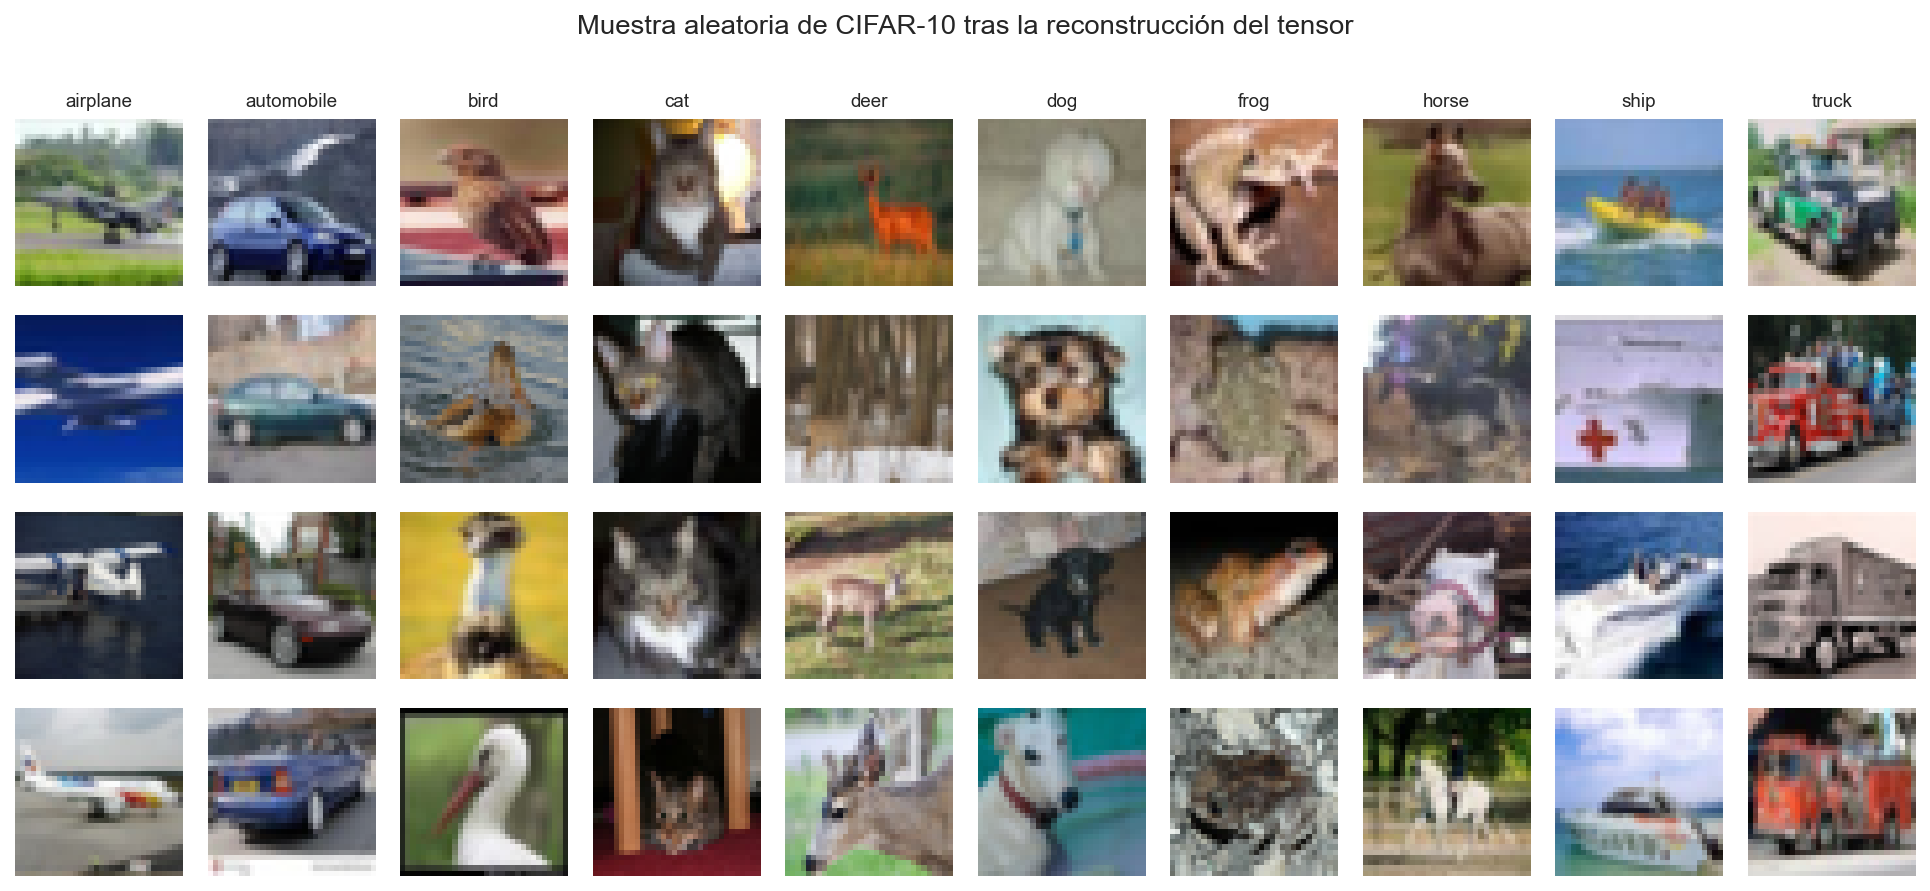
\includegraphics[width=0.9\textwidth]{fig02_muestra_imagenes.png}
\caption{Muestra aleatoria de imágenes de CIFAR-10 tras la reconstrucción del
tensor, con su etiqueta de clase. Sirve como verificación visual de que la
transposición de canales se realizó correctamente.}
\label{fig:muestra}
\end{figure}

%=====================  6. DESCRIPCIÓN  ==============================
\section{Descripción del conjunto de datos}

\subsection{A nivel de atributos}

La Tabla~\ref{tab:atributos} resume los atributos. Las tres primeras filas
corresponden a atributos originales; las restantes son derivadas en la etapa de
\emph{feature engineering}. Los valores numéricos deben completarse con la salida
de la celda correspondiente del \emph{notebook}.

{\scriptsize
\begin{longtable}{@{}p{1.9cm}p{2.6cm}p{1.7cm}p{1.2cm}p{1.9cm}p{1.1cm}p{2.1cm}p{1.9cm}@{}}
\toprule
\textbf{Atributo} & \textbf{Significado} & \textbf{Tipo} & \textbf{Nulos} & \textbf{Rango / valores únicos} & \textbf{Unidad} & \textbf{Distribución y estadísticos} & \textbf{Relevancia} \\
\midrule
\endfirsthead
\toprule
\textbf{Atributo} & \textbf{Significado} & \textbf{Tipo} & \textbf{Nulos} & \textbf{Rango} & \textbf{Unidad} & \textbf{Estadísticos} & \textbf{Relevancia} \\
\midrule
\endhead
\texttt{img\_id} & Identificador único de la imagen & Nominal (clave) & 0 (0\%) & 60\,000 únicos & --- & --- & Unión entre tablas \\
\texttt{clase} & Etiqueta semántica asignada por anotadores & Categórico nominal & 0 (0\%) & 10 valores & --- & Uniforme: 6\,000 por clase & H1, H2 \\
\texttt{split} & Partición original & Categórico nominal & 0 (0\%) & train / test & --- & 50\,000 / 10\,000 & Cruce con CIFAR-10H \\
\texttt{brillo} & Media del canal V (HSV) & Numérico continuo & 0 (0\%) & $[0.05, 0.99]$ & normalizado & $\bar{x}=0.540$, $\tilde{x}=0.535$, $\sigma=0.128$, IQR$=0.164$ (asim. 0.12) & H1, H2, H3 \\
\texttt{contraste} & Desviación estándar de la luminancia & Numérico continuo & 0 (0\%) & $[0.02, 0.45]$ & normalizado & $\bar{x}=0.196$, $\tilde{x}=0.195$, $\sigma=0.060$, IQR$=0.084$ (asim. 0.17) & H1, H2, H3 \\
\texttt{saturacion} & Media del canal S (HSV) & Numérico continuo & 0 (0\%) & $[0.00, 0.98]$ & normalizado & $\bar{x}=0.274$, $\tilde{x}=0.255$, $\sigma=0.141$, IQR$=0.185$ (asim. 0.73) & H1, H2 \\
\texttt{entropia} & Entropía de Shannon del histograma de grises & Numérico continuo & 0 (0\%) & $[0.81, 7.79]$ & bits & $\bar{x}=6.950$, $\tilde{x}=7.091$, $\sigma=0.579$, IQR$=0.587$ (asim. $-2.23$) & H1, H3 \\
\texttt{densidad\_bordes} & Proporción de píxeles de borde (Sobel) & Numérico continuo & 0 (0\%) & $[0.04, 0.99]$ & proporción & $\bar{x}=0.812$, $\tilde{x}=0.856$, $\sigma=0.144$, IQR$=0.161$ (asim. $-1.63$) & H1, H2 \\
\texttt{tono\_dominante} & Modo del canal H (HSV), discretizado en 12 sectores, entre píxeles con saturación $>0.15$ & Categórico ordinal & \emph{[completar: \% acromáticas]} & 12 sectores & grados & \emph{[completar: moda]} & H1 \\
\texttt{unif\_fondo} & $\sigma$ de la banda perimetral de 4 px & Numérico continuo & 0 (0\%) & $[0.00, 0.44]$ & normalizado & $\bar{x}=0.176$, $\tilde{x}=0.173$, $\sigma=0.070$, IQR$=0.098$ (asim. 0.25) & H2 \\
\texttt{energia\_central} & Razón entre varianza del centro $16{\times}16$ y del total & Numérico continuo & 0 (0\%) & $[0.00, 3.83]$ & razón & $\bar{x}=0.965$, $\tilde{x}=0.897$, $\sigma=0.481$, IQR$=0.604$ (asim. 1.04) & H2, H3 \\
\texttt{cluster\_k8} & Cluster asignado con $k=8$ & Categórico nominal & 0 (0\%) & 8 valores & --- & \emph{[completar]} & H1, H2, H3 \\
\texttt{cluster\_k18} & Cluster asignado con $k=18$ & Categórico nominal & 0 (0\%) & 18 valores & --- & \emph{[completar]} & H1, H2 \\
\texttt{entropia\_humana} & Entropía de la distribución de votos (CIFAR-10H) & Numérico continuo & \emph{[solo test]} & $[0,\log_2 10]$ & bits & \emph{[completar]} & H3 \\
\texttt{consenso} & Proporción de votos a la clase mayoritaria & Numérico continuo & \emph{[solo test]} & $[0.1,1]$ & proporción & \emph{[completar]} & H3 \\
\bottomrule
\caption{Resumen de atributos originales y derivados.}
\label{tab:atributos}
\end{longtable}
}

\paragraph{Medidas de posición y dispersión.} Para cada variable numérica se
reportan media, mediana, moda (sobre la versión discretizada), cuartiles
$Q_1, Q_2, Q_3$, desviación estándar, amplitud e intervalo intercuartílico
$IQR = Q_3 - Q_1$. La Figura~\ref{fig:distribuciones} presenta las
distribuciones y la Figura~\ref{fig:boxplots} los \emph{boxplots} con los
valores atípicos según el criterio $[Q_1 - 1.5\,IQR,\; Q_3 + 1.5\,IQR]$.

\begin{figure}[H]
\centering
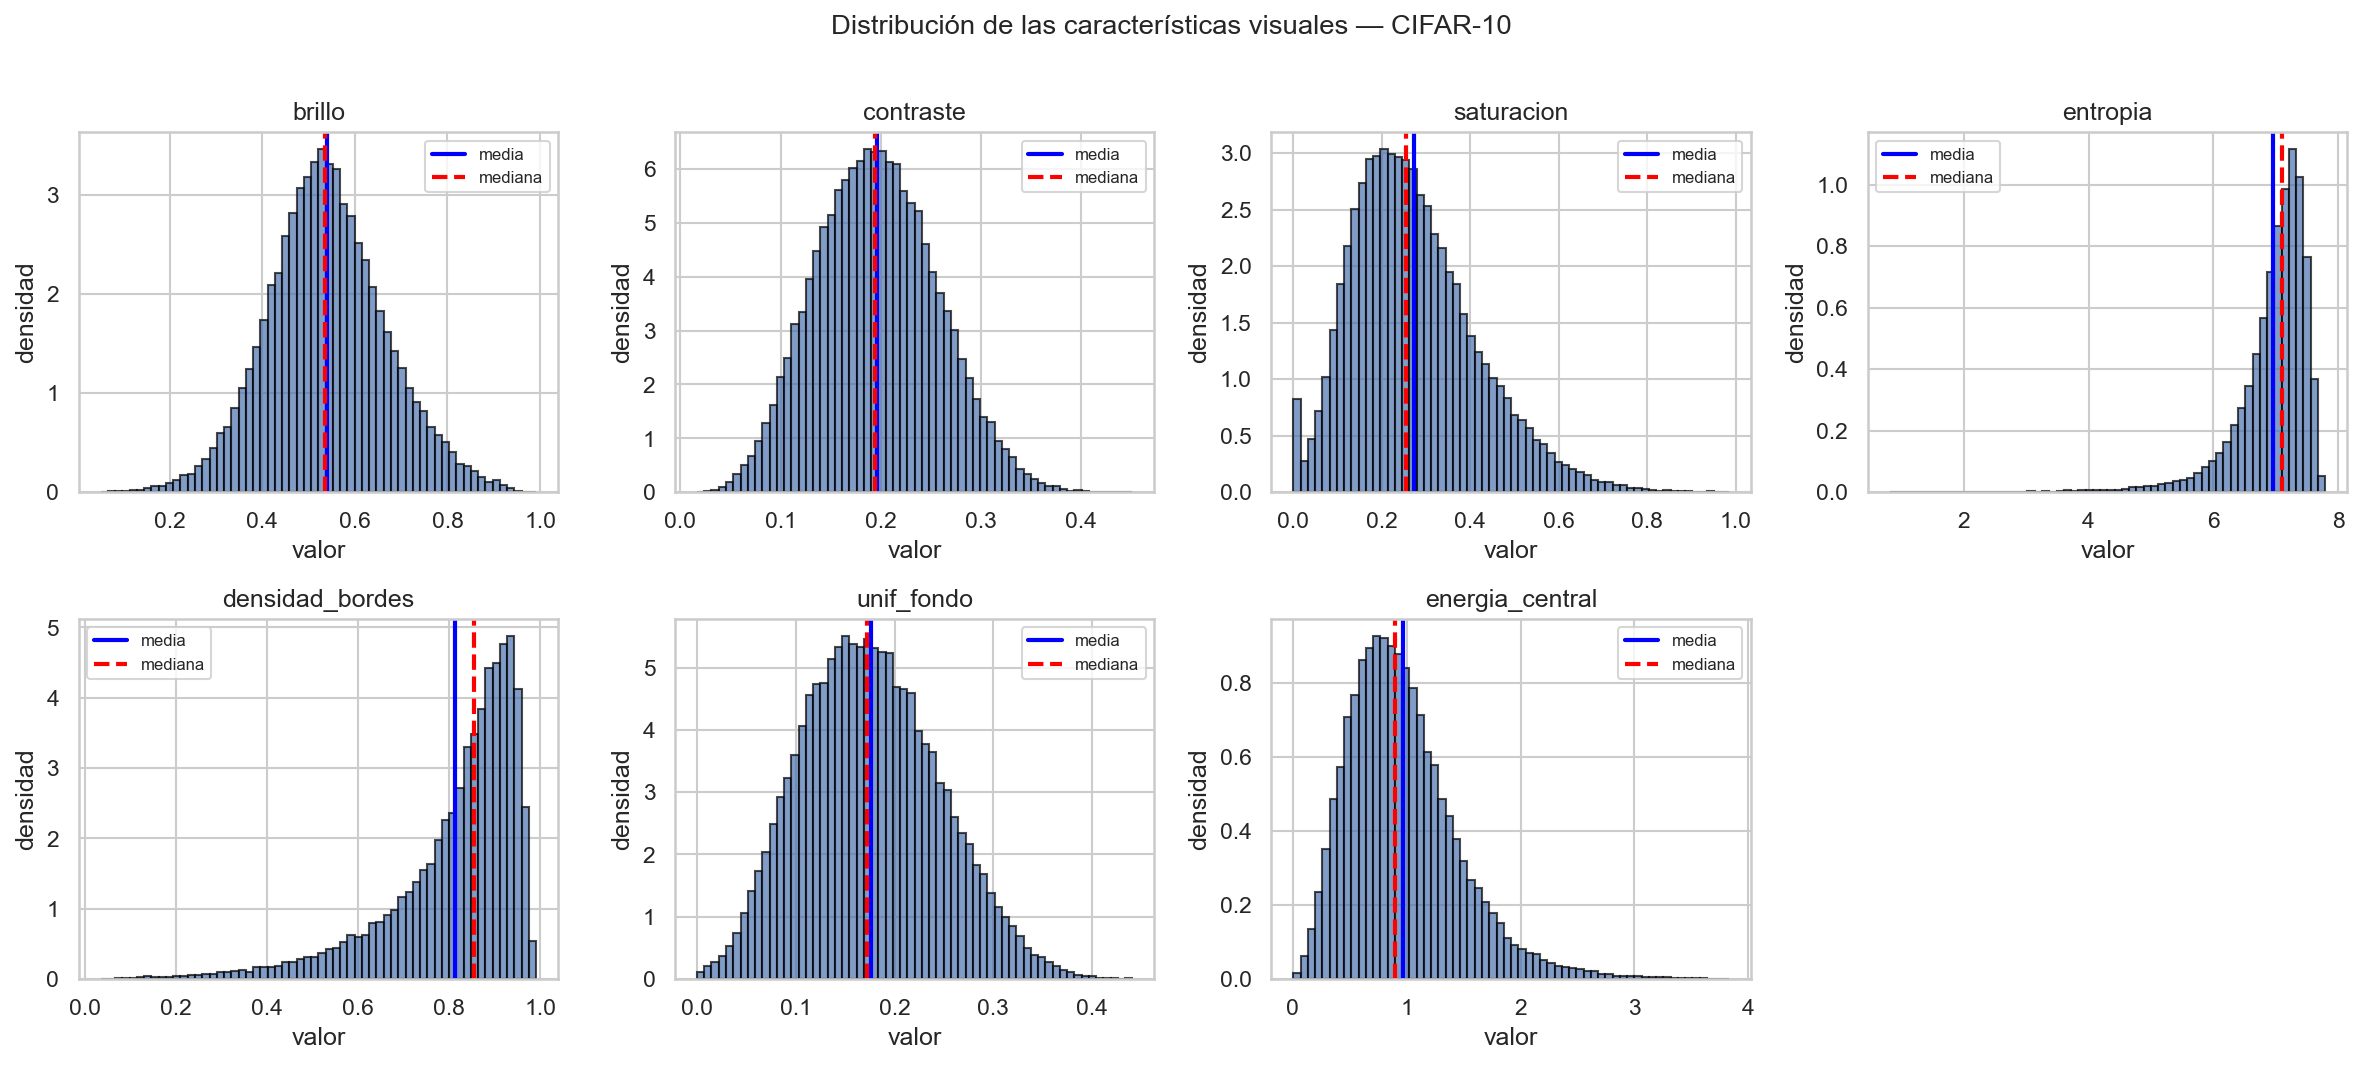
\includegraphics[width=\textwidth]{fig03_histogramas_caracteristicas.png}
\caption{Histogramas de las características visuales sobre CIFAR-10 completo, con
media (línea continua) y mediana (línea discontinua) superpuestas. Las
diferencias entre ambas medidas revelan la asimetría de cada distribución.}
\label{fig:distribuciones}
\end{figure}

\begin{figure}[H]
\centering
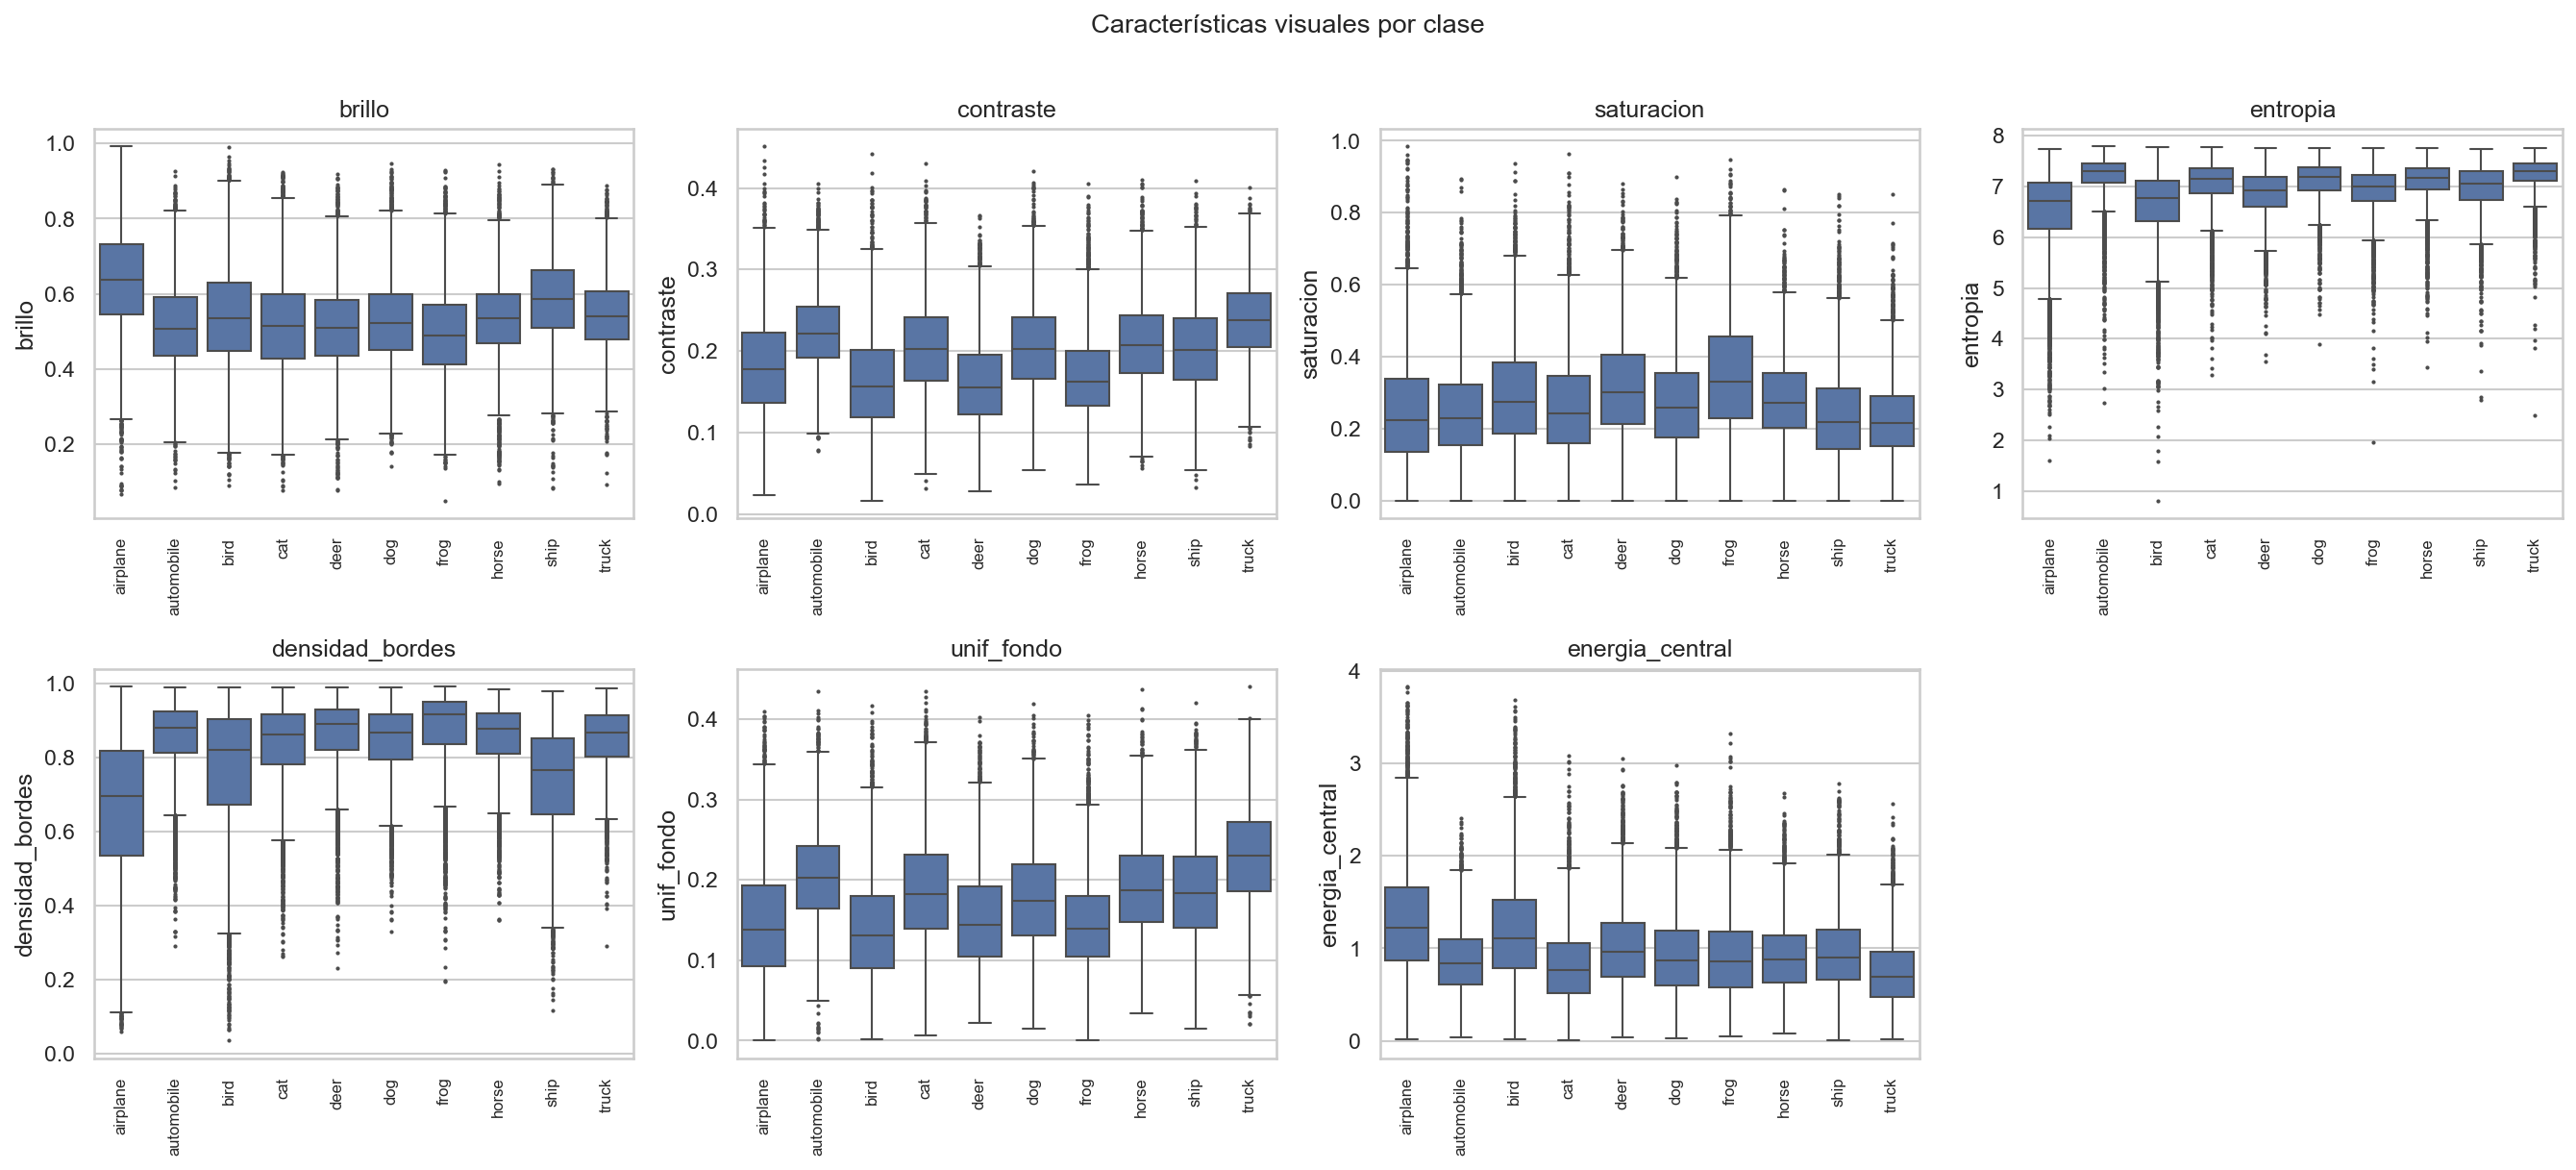
\includegraphics[width=\textwidth]{fig04_boxplots_por_clase.png}
\caption{Boxplots de cada característica visual desagregados por clase. Permiten
comparar simultáneamente la posición central, la dispersión y los valores
atípicos de las diez clases.}
\label{fig:boxplots}
\end{figure}

\subsection{A nivel de registros}

Cada fila representa \textbf{una imagen individual} de $32 \times 32$ píxeles en
tres canales RGB. La granularidad es, por tanto, la instancia: no hay agregación
temporal ni espacial, y no existen registros compuestos.

Las etiquetas corresponden a diez clases mutuamente excluyentes: \emph{airplane,
automobile, bird, cat, deer, dog, frog, horse, ship, truck}. El protocolo de
construcción del dataset garantiza que las clases son disjuntas (por ejemplo,
\emph{automobile} incluye sedanes y SUV pero excluye camionetas, que pertenecen a
\emph{truck}). El diseño es perfectamente balanceado: 6\,000 imágenes por clase,
de las cuales 5\,000 pertenecen al conjunto de entrenamiento y 1\,000 al de
prueba.

Tras incorporar el \emph{clustering}, cada registro adquiere una segunda
estructura de pertenencia --- el cluster --- que no coincide necesariamente con
la clase. La tensión entre ambas particiones es el objeto central de las
hipótesis 1 y 2.

\subsection{Relación entre atributos}

\begin{figure}[H]
\centering
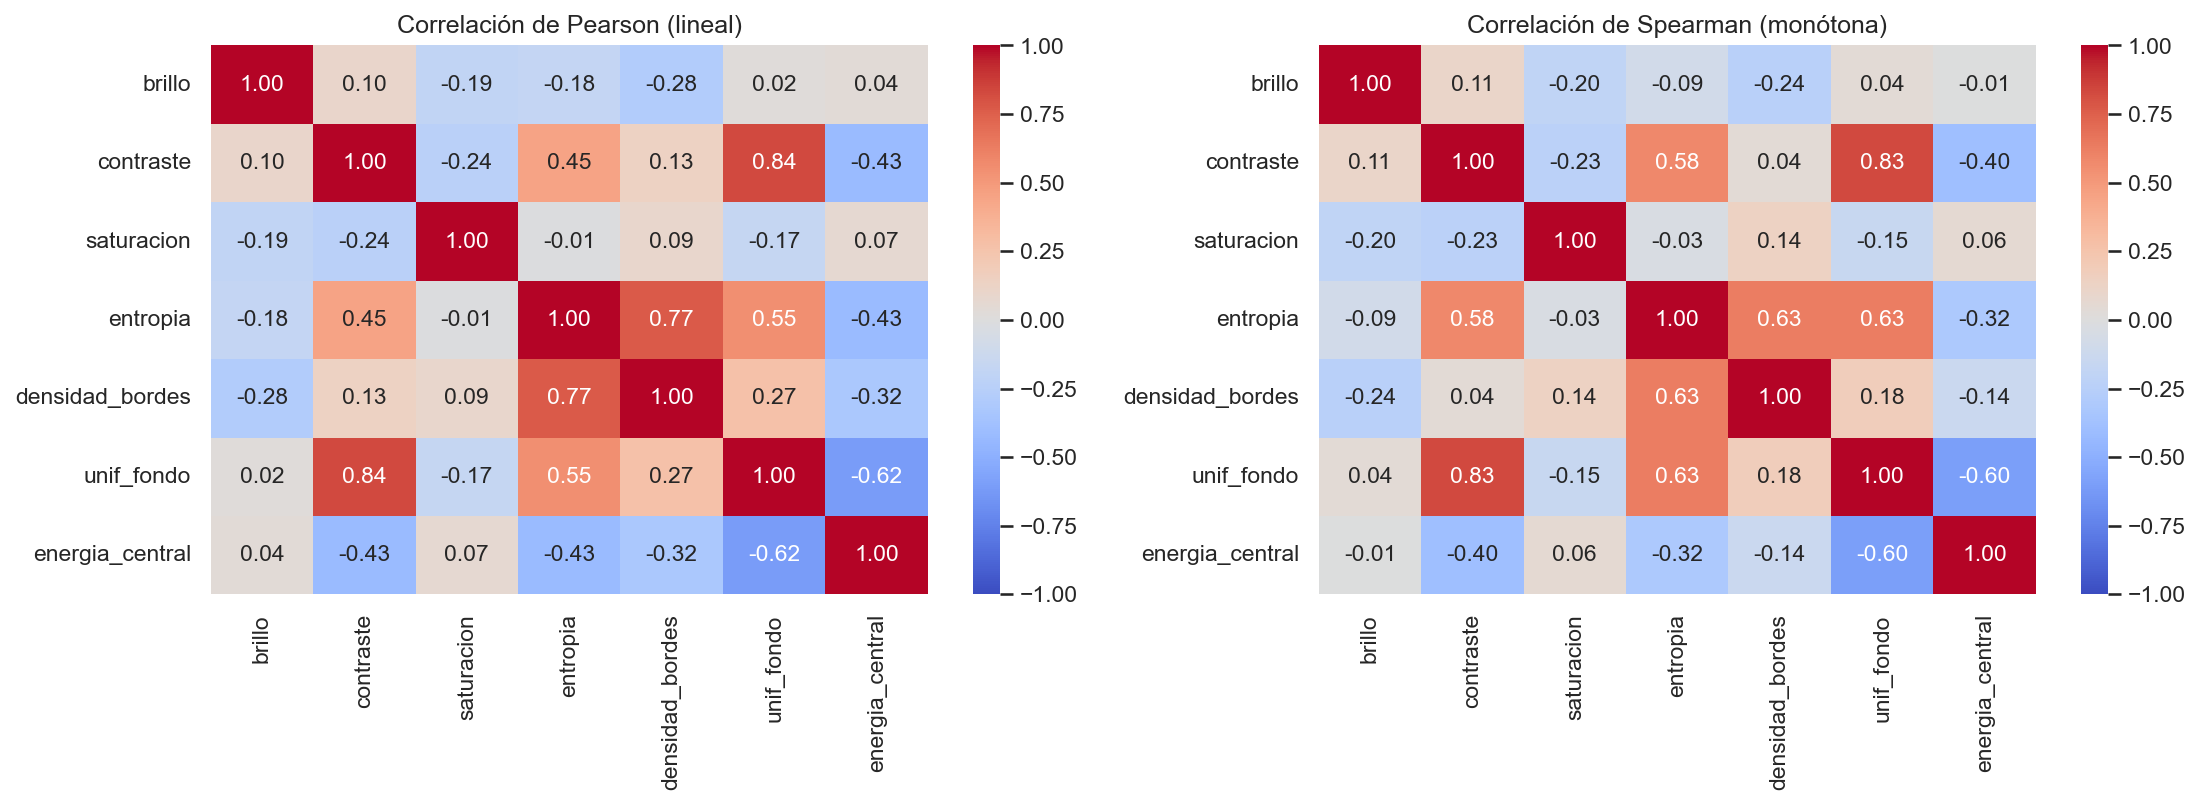
\includegraphics[width=0.8\textwidth]{fig05_matriz_correlacion.png}
\caption{Matriz de correlación de Pearson entre las características visuales.
Los colores cálidos indican asociación positiva y los fríos, negativa.}
\label{fig:corr}
\end{figure}

\begin{figure}[H]
\centering
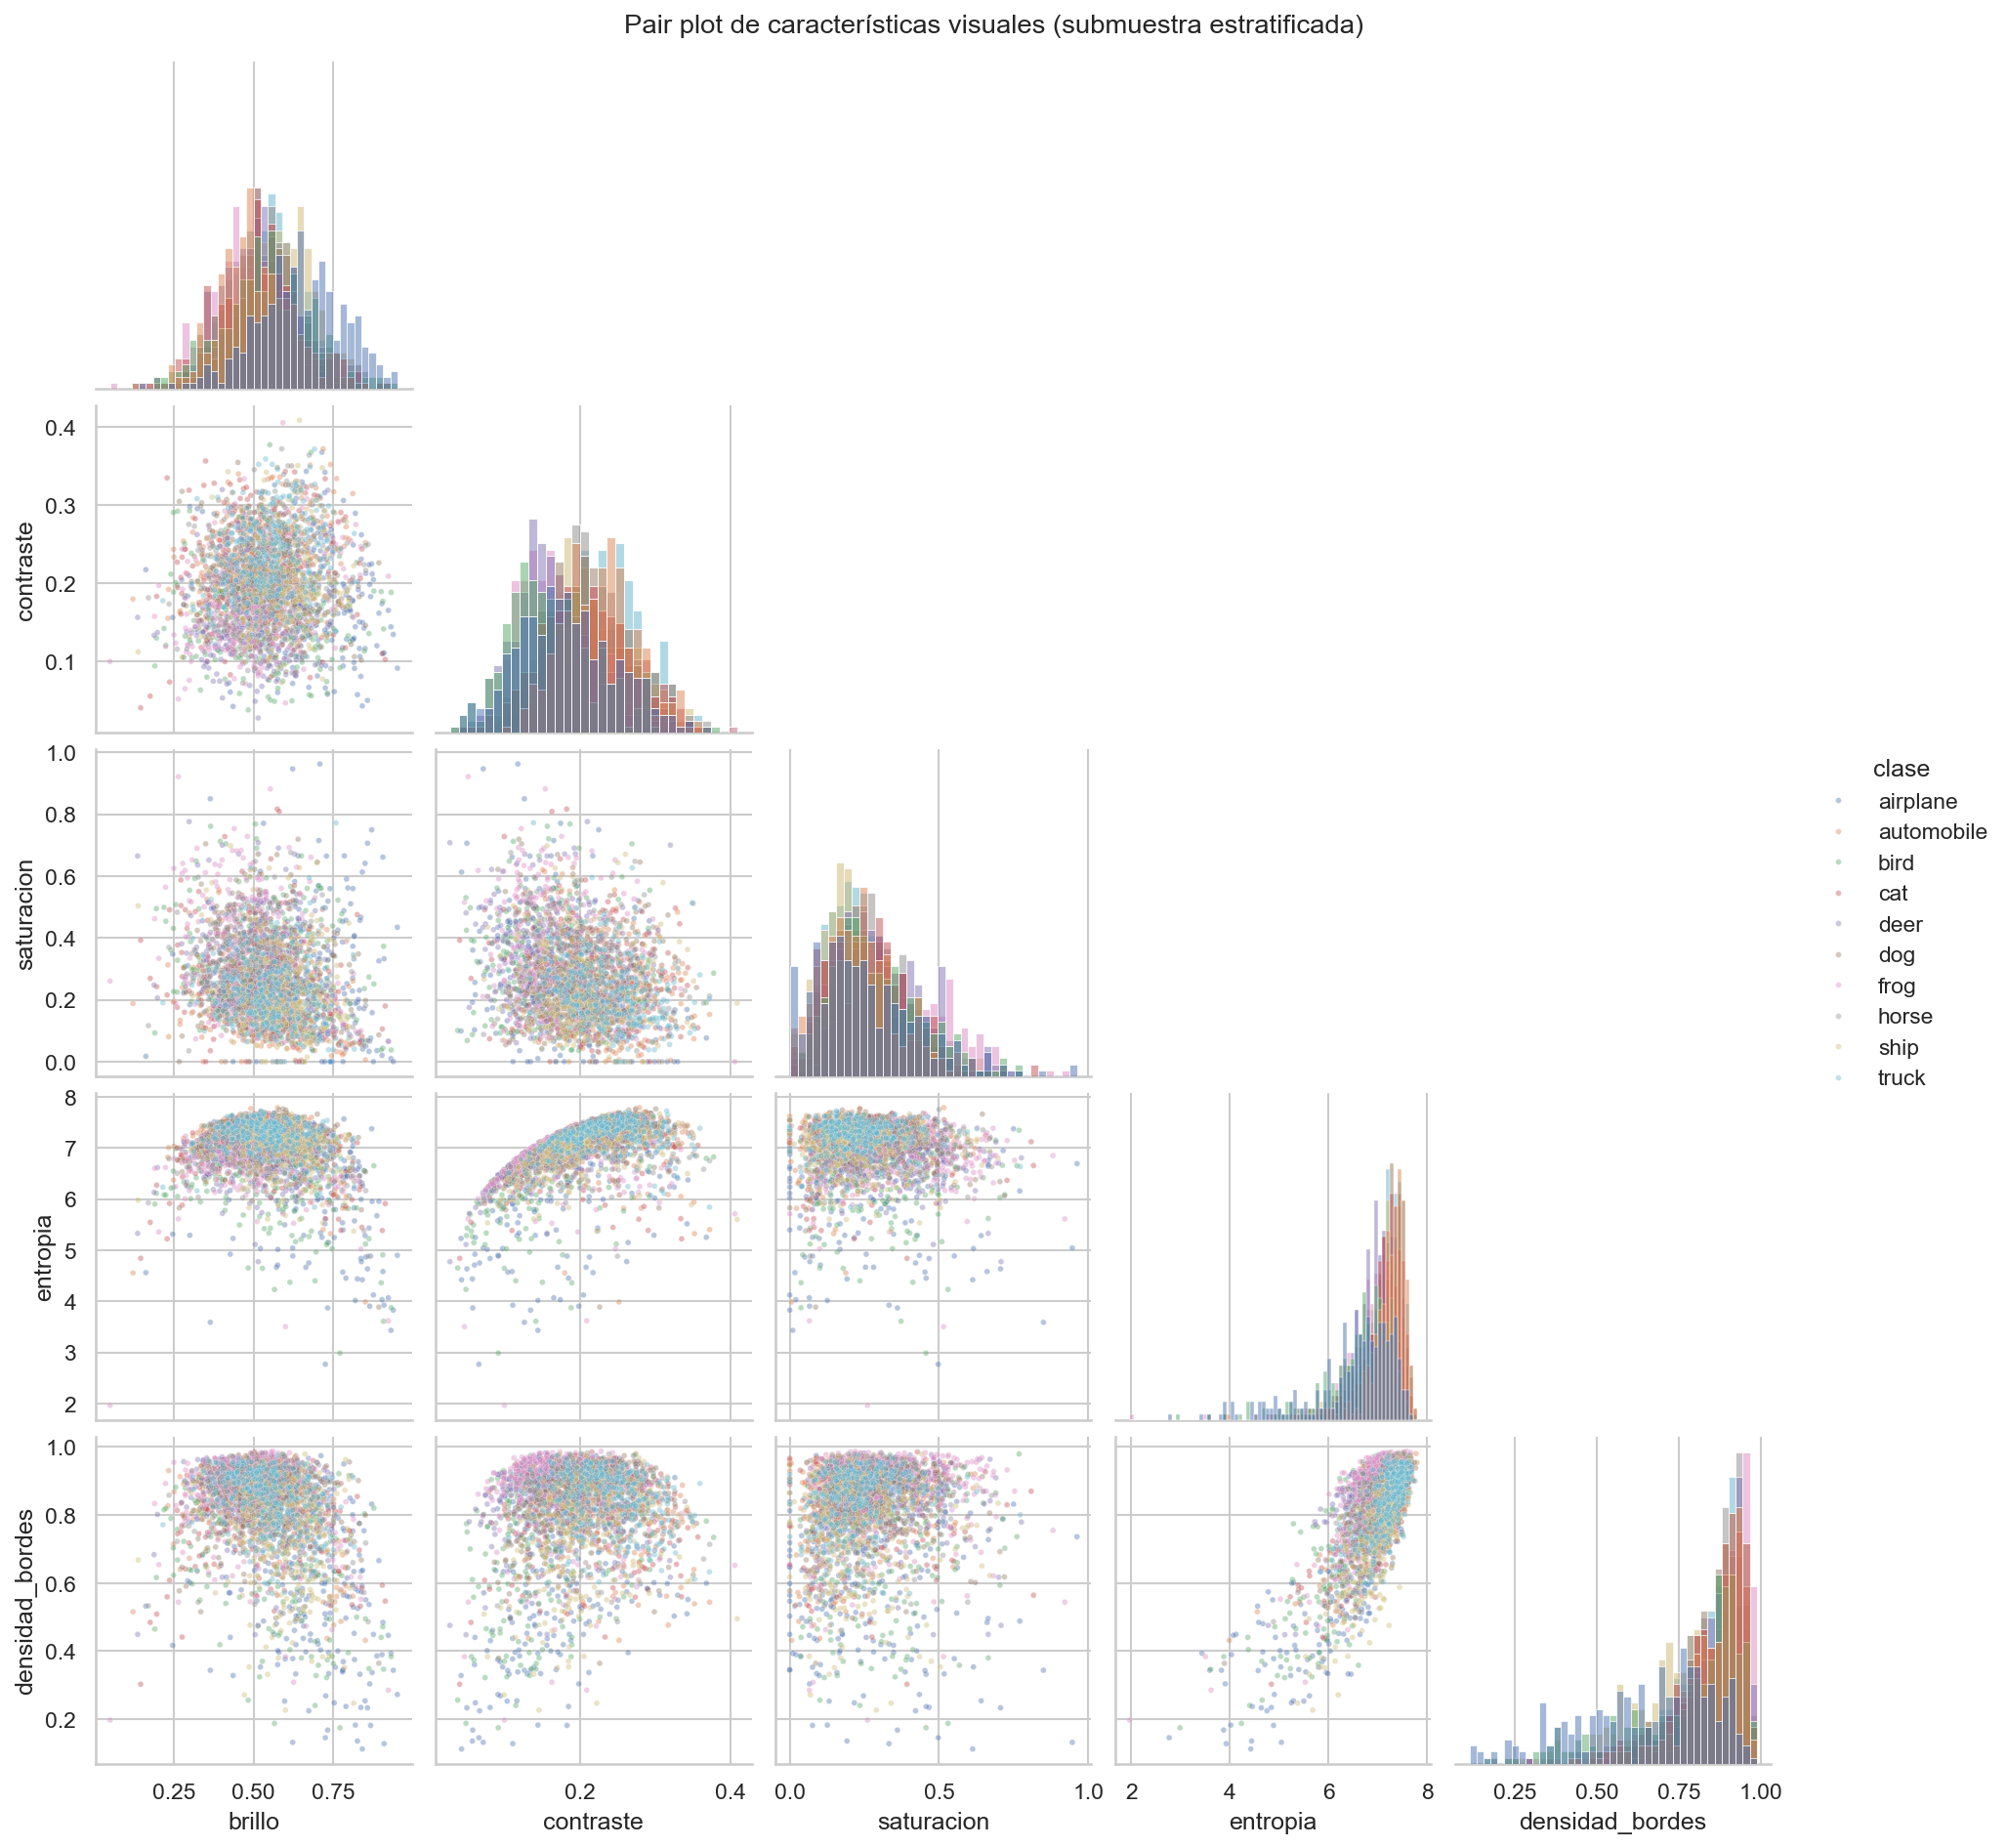
\includegraphics[width=\textwidth]{fig06_pairplot_caracteristicas.png}
\caption{Pair plot de las características visuales, coloreado por clase
(submuestra estratificada). La diagonal muestra las distribuciones marginales.}
\label{fig:pairplot}
\end{figure}

Se reportan tanto Pearson como Spearman, dado que varias relaciones esperadas son
monótonas pero no lineales (por ejemplo, entre entropía y densidad de bordes). La
comparación entre ambos coeficientes se presenta en la
Tabla~\ref{tab:correlaciones}.

\begin{table}[H]
\centering
\small
\begin{tabular}{@{}llccp{5.2cm}@{}}
\toprule
\textbf{Variable A} & \textbf{Variable B} & \textbf{Pearson} & \textbf{Spearman} & \textbf{Lectura} \\
\midrule
entropia & densidad\_bordes & $+0.770$ & $+0.630$ & Relación positiva fuerte y esperada; la brecha Pearson--Spearman ($0.14$) indica que parte de la asociación no es estrictamente lineal \\
unif\_fondo & densidad\_bordes & $+0.273$ & $+0.176$ & Positiva pero débil: un fondo no uniforme se asocia moderadamente con mayor densidad de bordes, no de forma determinista \\
energia\_central & contraste & $-0.428$ & $-0.395$ & Negativa moderada e inesperada: cuando la estructura se concentra en el centro de la imagen, el contraste global tiende a ser \emph{menor}, no mayor \\
saturacion & brillo & $-0.195$ & $-0.198$ & Negativa débil; imágenes más brillantes tienden levemente a estar menos saturadas (efecto de sobreexposición) \\
brillo & contraste & $+0.099$ & $+0.109$ & Prácticamente nula: ambas variables varían de forma esencialmente independiente \\
\bottomrule
\end{tabular}
\caption{Correlaciones más relevantes entre características visuales, calculadas
sobre las 60\,000 imágenes de CIFAR-10.}
\label{tab:correlaciones}
\end{table}

\paragraph{Relaciones inesperadas.} La correlación negativa entre
\texttt{energia\_central} y \texttt{contraste} ($\rho_{\text{Pearson}}=-0.428$)
no era la esperada: se anticipaba que un objeto central bien definido (alta
\texttt{energia\_central}) coincidiera con mayor contraste global, no con menor.
Una lectura plausible es que las imágenes con fondos muy texturizados elevan el
contraste \emph{global} sin que el objeto central concentre esa variación,
mientras que las imágenes con un objeto central nítido sobre un fondo liso
mantienen baja varianza fuera del centro y, por tanto, contraste global menor.
Antes de aceptar esta lectura, esta relación se inspeccionó mediante scatterplot
(incluido en el pair plot de la Figura~\ref{fig:pairplot}) para descartar que
fuera un artefacto de unos pocos puntos extremos, siguiendo la lección del
cuarteto de Anscombe.

\paragraph{Variables aparentemente independientes.} \texttt{brillo} y
\texttt{contraste} muestran una correlación prácticamente nula
($\rho_{\text{Pearson}}=+0.099$, $\rho_{\text{Spearman}}=+0.109$): el nivel de
iluminación de una imagen de CIFAR-10 no predice su nivel de contraste. Esto es
relevante para el diseño de la herramienta de Visual Analytics: ambas variables
aportan información no redundante y ninguna puede usarse como sustituto de la
otra.

%=====================  7. PROBLEMAS Y TRANSFORMACIONES  =============
\section{Problemas identificados y transformaciones (data wrangling)}

\subsection{Problemas detectados en los datos}

\begin{enumerate}[leftmargin=*]
  \item \textbf{Formato serializado no estándar.} Los datos no vienen en CSV ni
  en un formato tabular; requieren deserialización con \texttt{pickle} en modo
  \emph{bytes} y reordenamiento de ejes.
  \item \textbf{Ausencia total de atributos.} Salvo la etiqueta, no existe
  ninguna variable sobre la cual filtrar, agrupar u ordenar. Este es el problema
  estructural del dataset.
  \item \textbf{Posibles imágenes duplicadas o casi-duplicadas.} La literatura
  reporta solapamientos entre los conjuntos de entrenamiento y prueba de CIFAR,
  herencia de la recolección automática desde buscadores web. Una búsqueda por
  \emph{hash} MD5 exacto sobre las 60\,000 imágenes no encontró ningún
  duplicado bit-idéntico, lo cual es esperable: el fenómeno reportado en la
  literatura corresponde a \emph{casi}-duplicados (recortes, reescalados o
  recompresiones de una misma imagen de origen), no a copias exactas. Detectar
  esos casos requeriría un \emph{hash} perceptual (p.\,ej.\ \emph{difference
  hashing}), que queda fuera del alcance de esta etapa.
  \item \textbf{Errores de etiquetado.} Trabajos de auditoría sobre
  \emph{benchmarks} han documentado etiquetas incorrectas en los conjuntos de
  prueba de CIFAR. CIFAR-10H permite detectarlos indirectamente mediante el
  desacuerdo humano.
  \item \textbf{Escalas heterogéneas entre características derivadas.} La
  entropía se mide en bits ($[0,8]$), la densidad de bordes es una proporción
  ($[0,1]$) y el contraste una desviación estándar. Sin normalización, las
  distancias y el \emph{clustering} quedarían dominados por la entropía.
  \item \textbf{Valores atípicos en las características derivadas.} Imágenes casi
  monocromáticas producen contraste y entropía cercanos a cero; imágenes muy
  texturizadas saturan la densidad de bordes.
  \item \textbf{Imágenes degeneradas.} Un subconjunto pequeño puede presentar
  varianza nula o cercana a cero en uno o más canales.
  \item \textbf{Redundancia entre características.} Se anticipa colinealidad
  entre entropía, densidad de bordes y contraste.
  \item \textbf{Desalineación de índices en el cruce externo.} El orden de filas
  de CIFAR-10H no corresponde al orden del \texttt{test\_batch}.
  \item \textbf{Costo computacional.} La extracción de \emph{embeddings} sobre
  60\,000 imágenes y el \emph{clustering} aglomerativo, cuyo costo temporal es
  $O(n^2)$ en el mejor caso optimizado, obligan a planificar el uso de GPU y a
  cachear resultados intermedios.
\end{enumerate}

\subsection{Transformaciones realizadas}

{\small
\begin{longtable}{@{}p{3.3cm}p{4.2cm}p{4.2cm}p{3.2cm}@{}}
\toprule
\textbf{Problema} & \textbf{Transformación aplicada} & \textbf{Justificación} & \textbf{Resultado} \\
\midrule
\endfirsthead
\toprule
\textbf{Problema} & \textbf{Transformación} & \textbf{Justificación} & \textbf{Resultado} \\
\midrule
\endhead
(1) Formato serializado & Deserialización y \texttt{transpose} a formato HWC; volcado a Parquet & Parquet permite lectura columnar rápida y preserva tipos & Tabla única reproducible \\
(2) Ausencia de atributos & \emph{Feature engineering}: creación de 8 variables visuales interpretables & Dotar al dataset de atributos sobre los cuales aplicar operaciones tabulares & De 1 a 9 atributos por imagen \\
(3) Duplicados & Detección por \emph{hash} MD5 exacto sobre el tensor de píxeles & Los duplicados exactos inflarían artificialmente el tamaño de los clusters & 0 encontrados sobre 60\,000 imágenes \\
(5) Escalas heterogéneas & Estandarización $z$-score sobre las variables continuas & Evita que una variable domine las distancias por su rango & Variables comparables \\
(6) Valores atípicos & Marcado (no eliminación) mediante criterio $1.5\,IQR$ & Los extremos son informativos: señalan imágenes de baja calidad, que interesan al análisis & Columna \texttt{es\_atipico} \\
(7) Imágenes degeneradas & Marcado de registros con contraste $<10^{-3}$ (varianza casi nula) & No aportan información y distorsionan los estadísticos & 0 encontradas sobre 60\,000 imágenes \\
(8) Redundancia & Análisis de correlación previo a cualquier reducción; PCA solo con fines de visualización & Conservar la interpretabilidad es el objetivo del trabajo & Conjunto reducido justificado \\
(9) Desalineación de índices & Unión explícita por \texttt{img\_id} y validación cruzada con la clase mayoritaria & Una unión posicional produciría un cruce silenciosamente incorrecto & Unión verificada \\
--- & Discretización de \texttt{tono\_dominante} en 12 sectores & Facilita el análisis categórico y el futuro filtrado en la interfaz & Variable ordinal \\
--- & Codificación de \texttt{clase} y \texttt{cluster} como categóricas & Reduce memoria y habilita tablas de contingencia & --- \\
\bottomrule
\caption{Transformaciones aplicadas, su justificación y su resultado.}
\label{tab:transformaciones}
\end{longtable}
}

\begin{figure}[H]
\centering
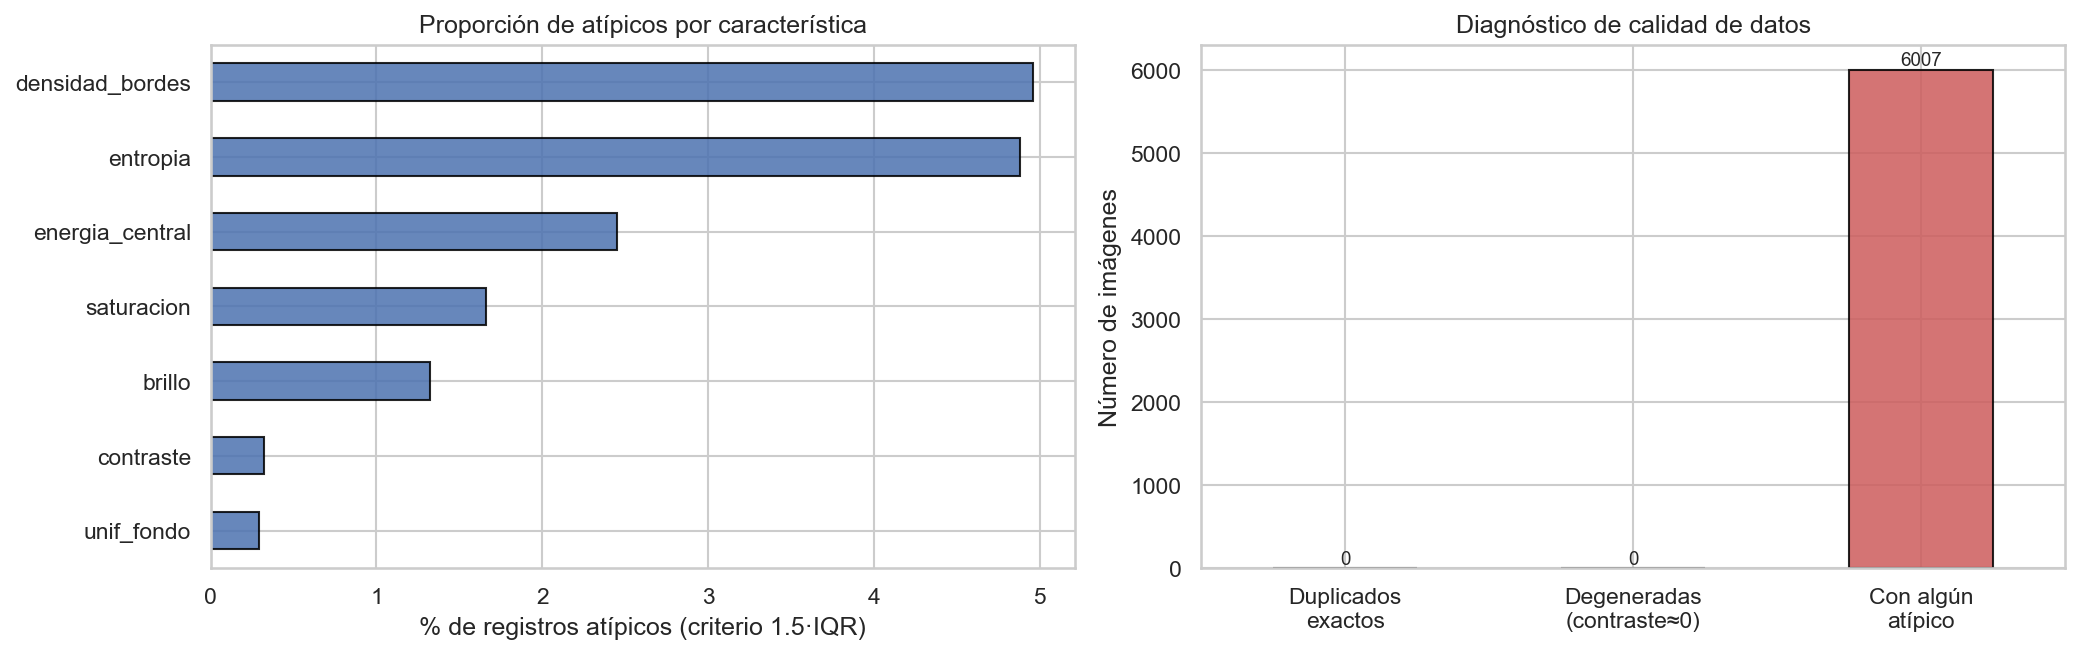
\includegraphics[width=0.85\textwidth]{fig07_calidad_datos.png}
\caption{Diagnóstico de calidad de datos: conteo de duplicados detectados,
imágenes degeneradas y proporción de valores atípicos por característica.}
\label{fig:calidad}
\end{figure}

%=====================  8. EXPLORACIÓN  ==============================
\section{Exploración y respuesta a las hipótesis}

\subsection{Hipótesis 1: confluencia visual entre clases}

\begin{figure}[H]
\centering
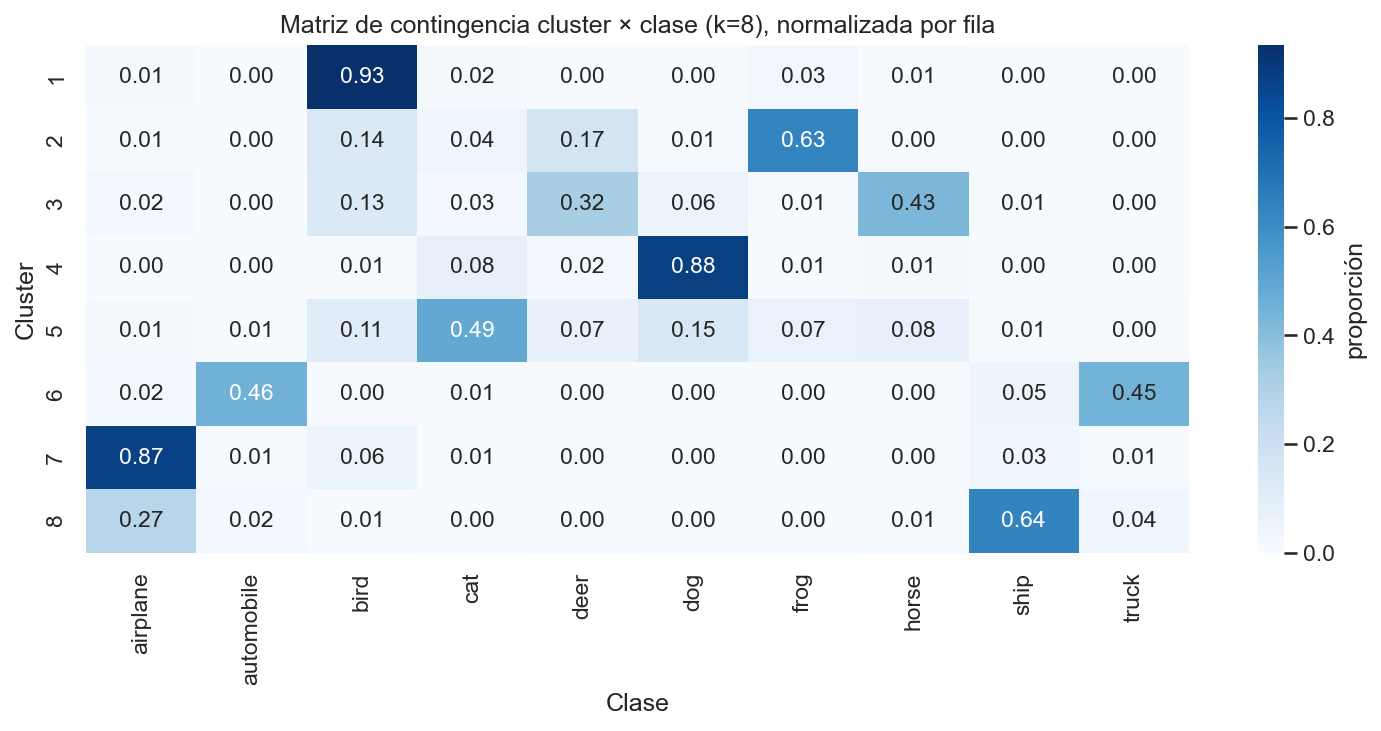
\includegraphics[width=0.9\textwidth]{fig08_h1_matriz_clase_cluster.png}
\caption{Matriz de contingencia clase $\times$ cluster ($k=8$), normalizada por
fila. Las celdas oscuras en columnas compartidas identifican clusters que reúnen
más de una clase semántica.}
\label{fig:h1a}
\end{figure}

\emph{Descripción e interpretación.} Con $k=8$ clusters, la pureza (proporción de
la clase mayoritaria dentro del cluster) va de $0.93$ en el cluster más
homogéneo hasta $0.43$ en el más mixto. Tres clusters caen por debajo del
umbral de $0.6$: el 3 (pureza $0.427$), el 6 (pureza $0.456$) y el 5 (pureza
$0.491$). En conjunto reúnen una fracción considerable del dataset y mezclan
clases sin relación semántica evidente entre sí, lo que descarta que el
agrupamiento se explique trivialmente por similitud de etiqueta.

\begin{figure}[H]
\centering
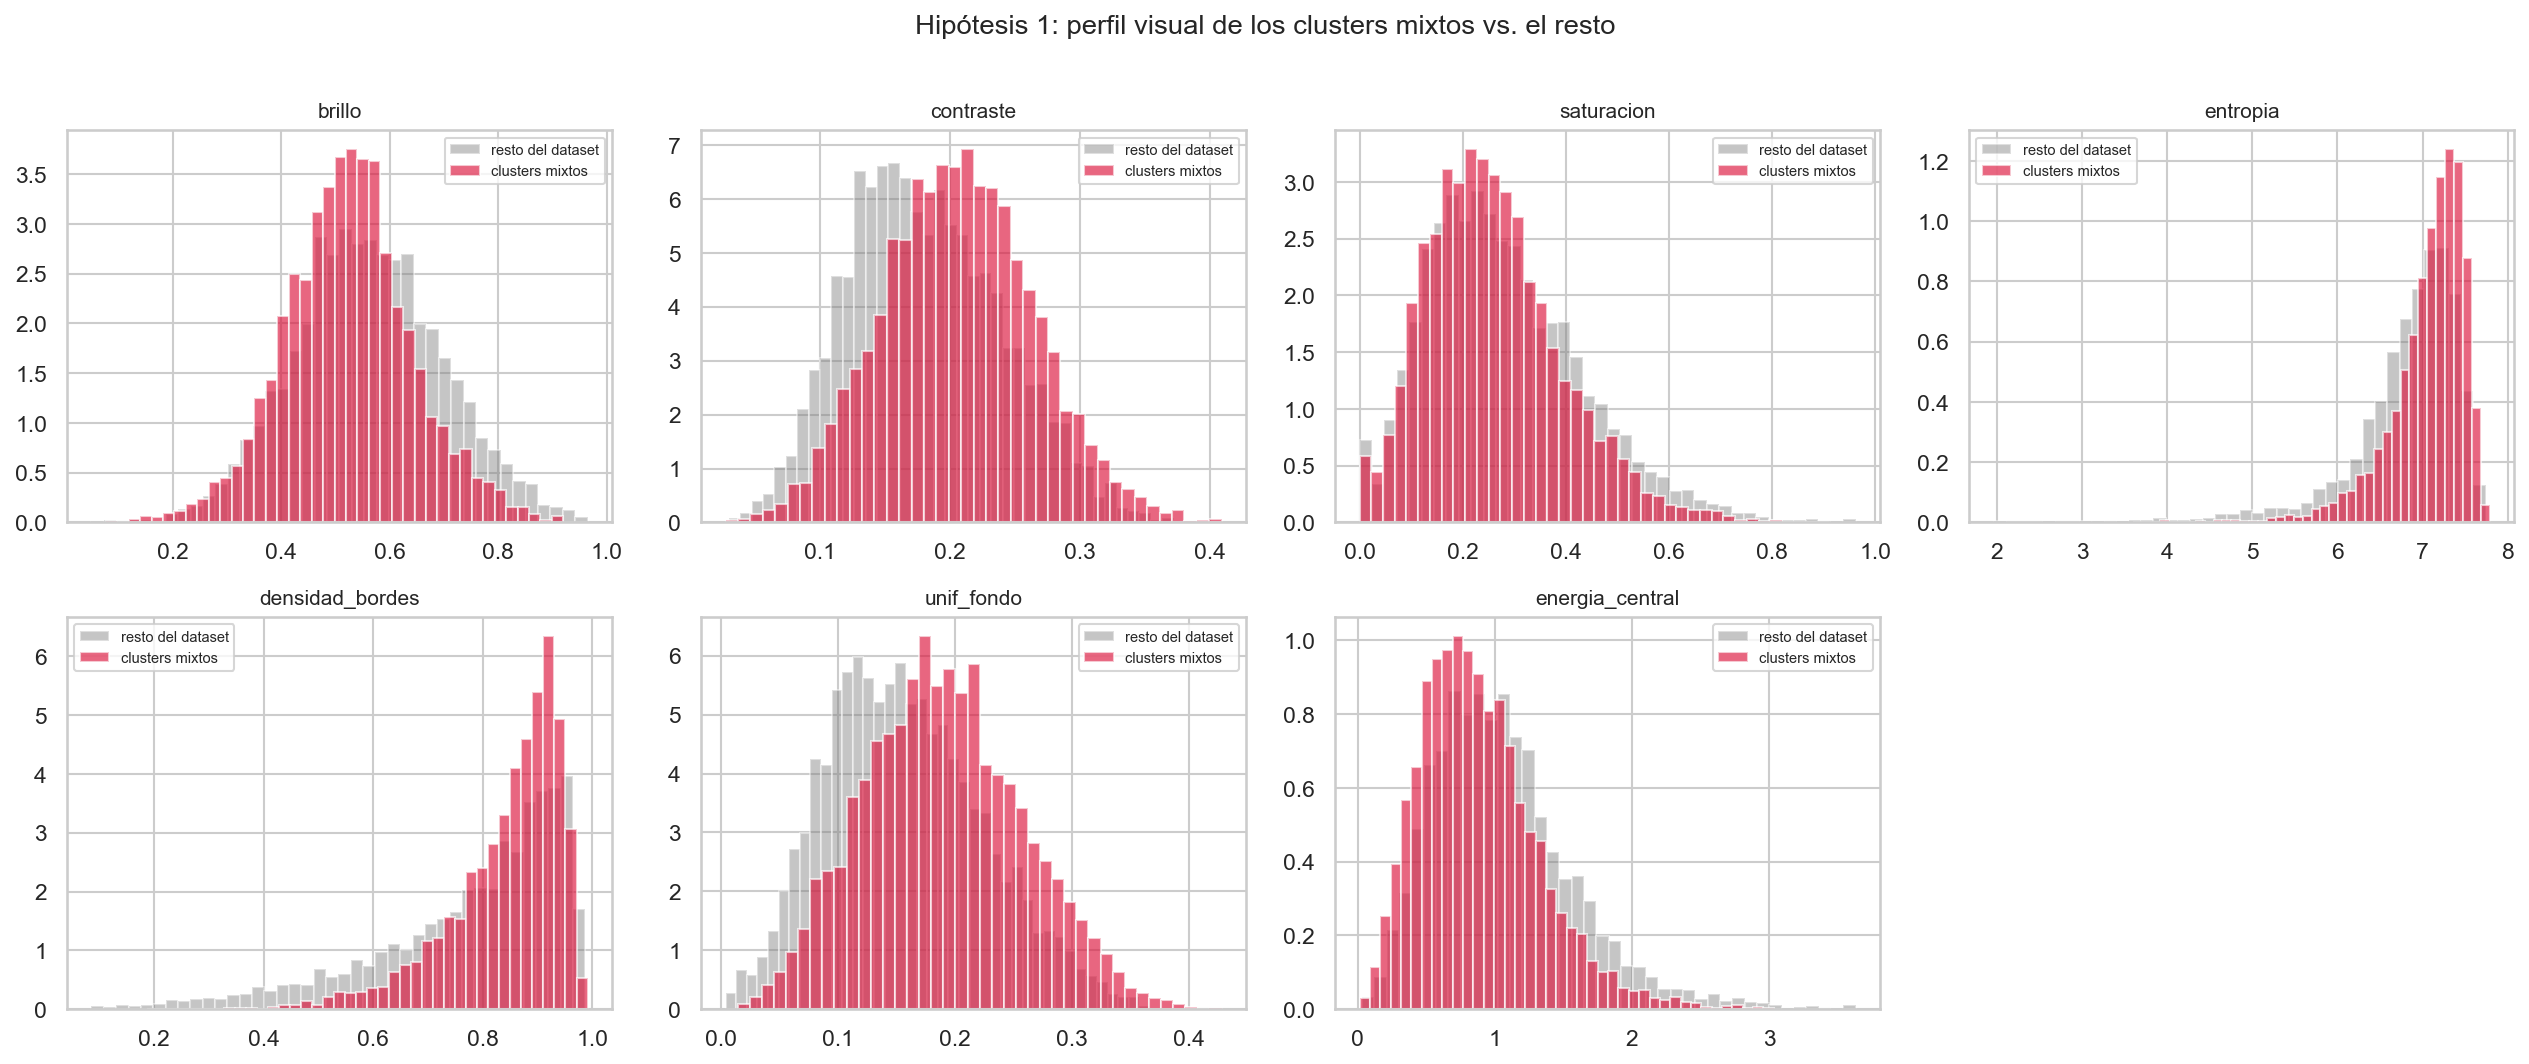
\includegraphics[width=\textwidth]{fig09_h1_perfil_clusters.png}
\caption{Perfil de características visuales de los clusters mixtos frente al
resto del dataset. Cada panel muestra la distribución de una característica
dentro del cluster (color) y en el dataset completo (gris).}
\label{fig:h1b}
\end{figure}

\emph{Descripción e interpretación.} El tamaño del efecto ($d$ de Cohen) entre los
clusters mixtos $\{3,5,6\}$ y el resto del dataset es mayor para
\texttt{unif\_fondo} ($d=+0.490$), \texttt{densidad\_bordes} ($d=+0.476$) y
\texttt{entropia} ($d=+0.465$), seguidos de \texttt{contraste} ($d=+0.432$) y
\texttt{energia\_central} ($d=-0.368$). Todos son efectos de magnitud media según
la convención de Cohen. La lectura conjunta es consistente: las imágenes que
confluyen entre clases distintas comparten fondos poco uniformes, mayor
densidad de bordes y mayor entropía --- es decir, comparten \emph{complejidad
visual}, no una paleta de color ni una clase semántica particular.

\paragraph{Conclusión intermedia H1.} \textbf{Se confirma.} Existen clusters del
dendrograma ($k=8$) que agrupan imágenes de clases semánticamente distintas
(pureza $<0.6$ en 3 de 8 clusters), y ese agrupamiento resulta explicable
mediante características visuales cuantificables: los clusters mixtos se
distinguen del resto principalmente por mayor \texttt{unif\_fondo},
\texttt{densidad\_bordes} y \texttt{entropia}, con tamaños de efecto medios
($d\approx 0.4$--$0.5$). Las clases confluyen cuando comparten complejidad de
fondo y textura, no necesariamente color o forma del objeto.

\subsection{Hipótesis 2: divergencia visual dentro de una clase}

\begin{figure}[H]
\centering
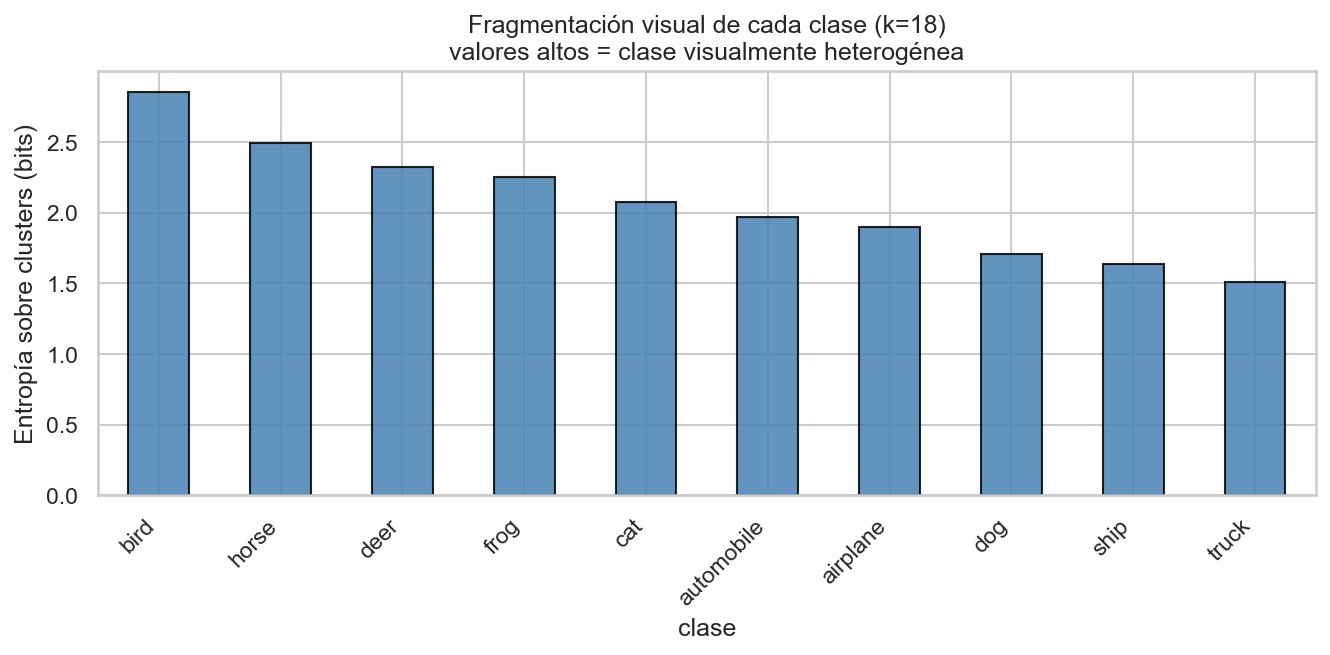
\includegraphics[width=0.9\textwidth]{fig10_h2_fragmentacion_clases.png}
\caption{Grado de fragmentación de cada clase a través de los clusters, medido
mediante la entropía de la distribución de la clase sobre los clusters. Valores
altos indican clases visualmente heterogéneas.}
\label{fig:h2a}
\end{figure}

\begin{figure}[H]
\centering
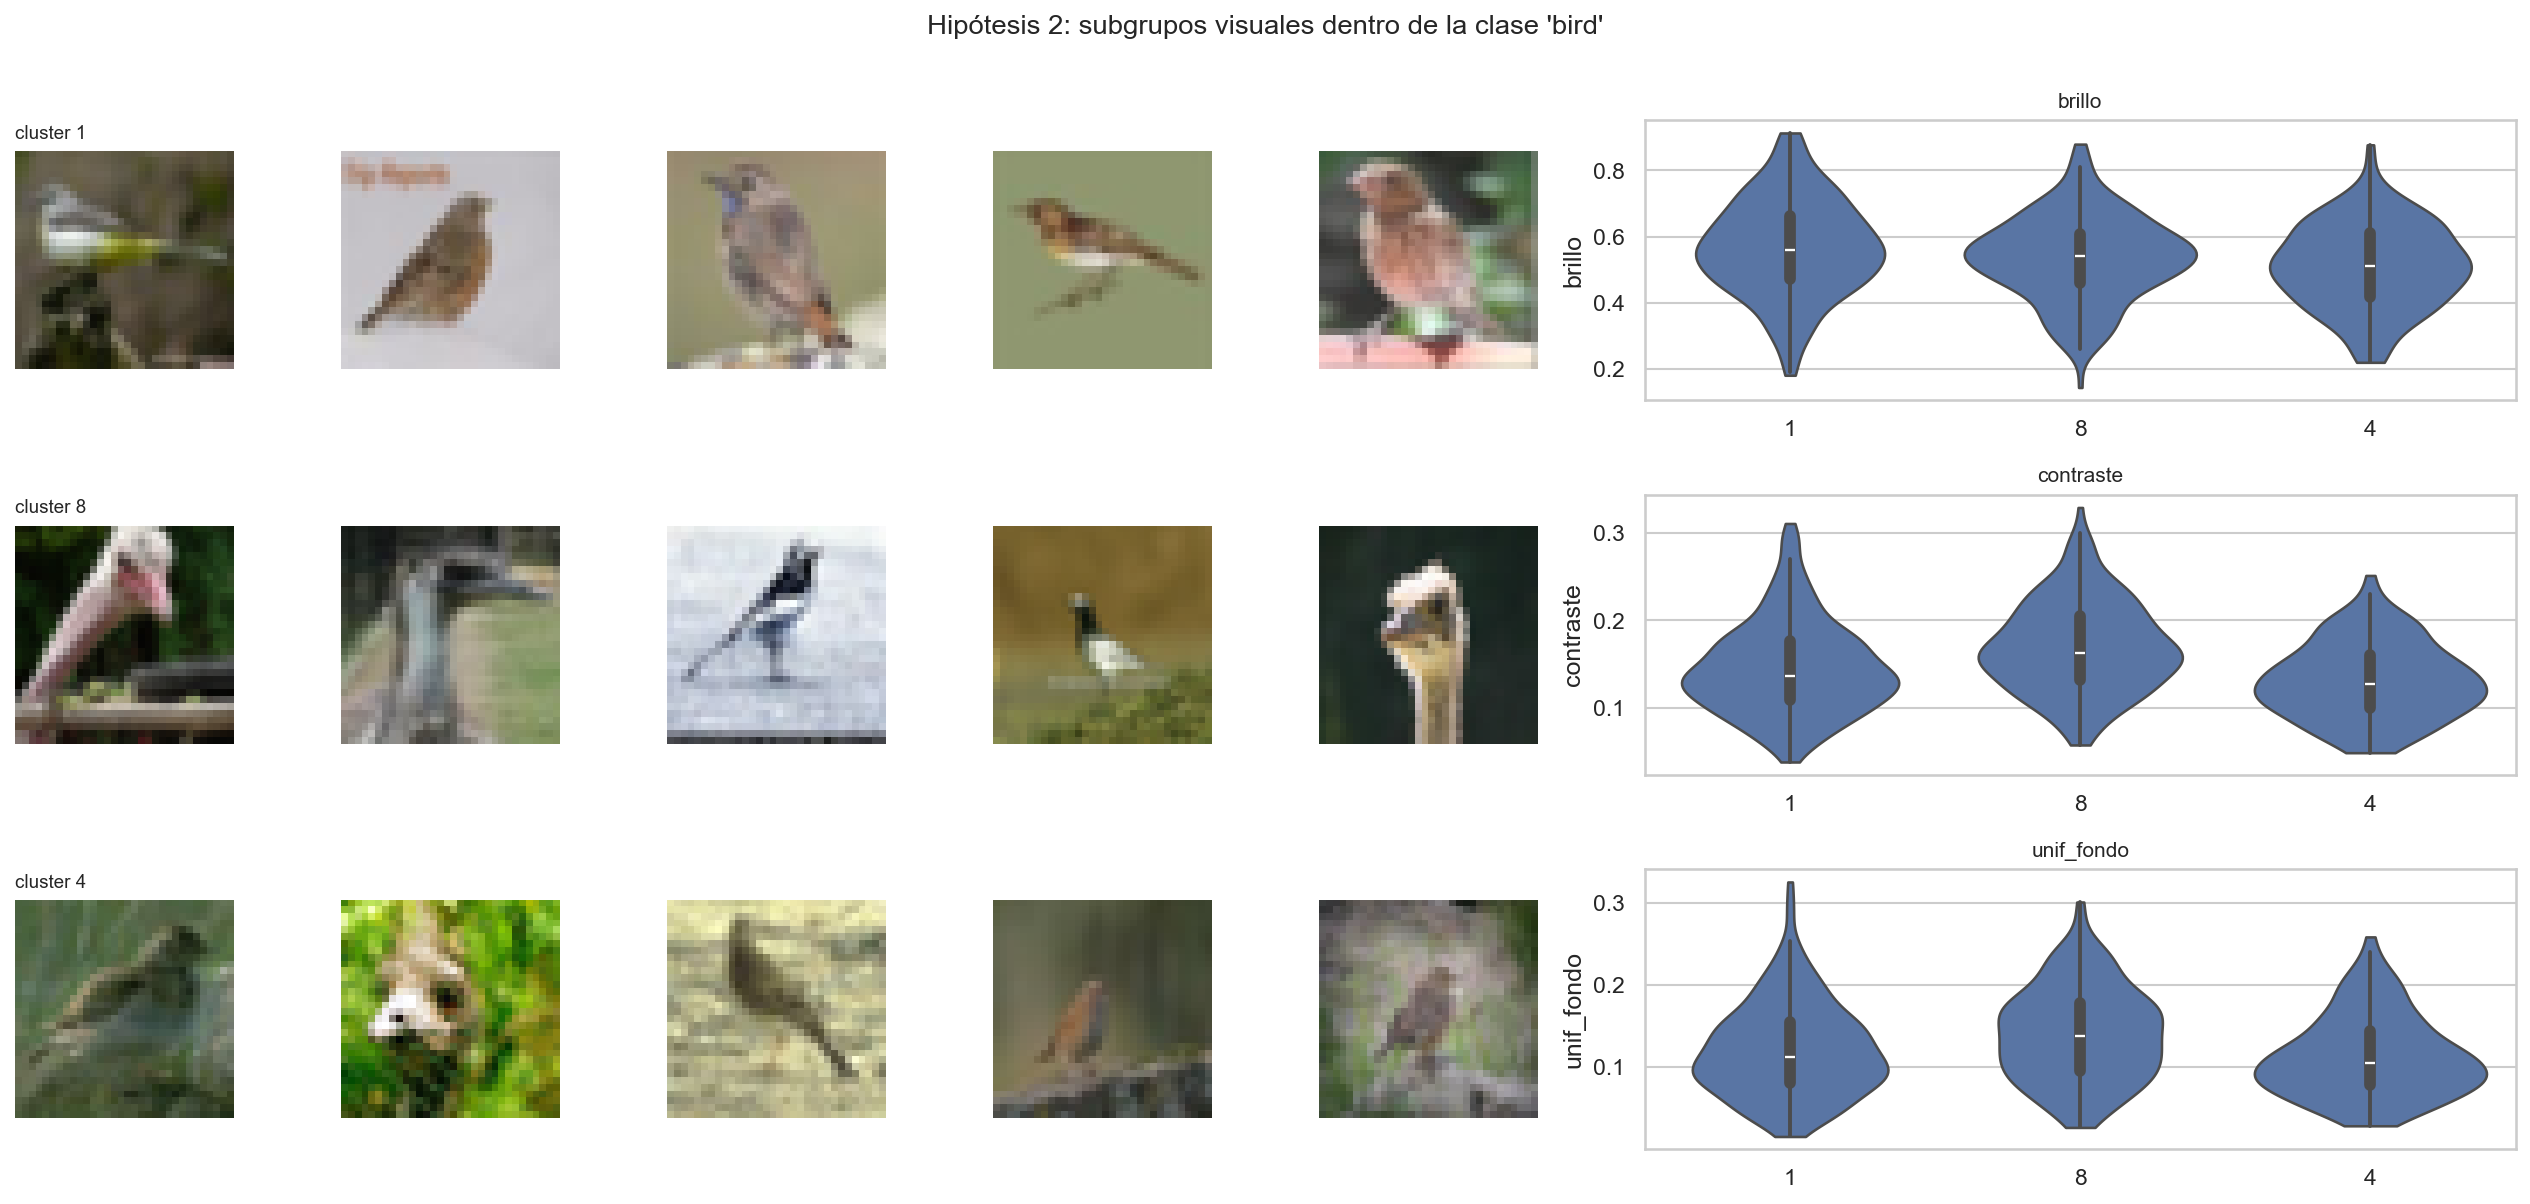
\includegraphics[width=\textwidth]{fig11_h2_subgrupos_clase.png}
\caption{Para la clase con mayor fragmentación: mosaico de imágenes
representativas de cada subgrupo junto a los violin plots de las características
que mejor los separan.}
\label{fig:h2b}
\end{figure}

\emph{Descripción e interpretación.} La clase con mayor entropía de distribución
sobre los 18 clusters ---y por tanto la más fragmentada visualmente--- es
\emph{bird}. A diferencia de clases con una pose y encuadre más homogéneos
(p.\,ej.\ \emph{automobile}), las aves aparecen en vuelo, posadas, sobre fondos
de cielo, agua o follaje, y a escalas muy distintas dentro del cuadro, lo cual
explica que su distribución sobre los clusters sea más pareja en lugar de
concentrarse en uno o dos.

\paragraph{Conclusión intermedia H2.} \textbf{Se confirma.} Al menos una clase
de CIFAR-10 --- \emph{bird} --- se fragmenta en múltiples subgrupos visualmente
diferenciados en lugar de concentrarse en un único cluster, lo que indica que su
etiqueta semántica agrupa patrones visuales heterogéneos. Esto valida que la
partición por clase y la partición por cluster capturan estructuras distintas y
complementarias del dataset.

\subsection{Hipótesis 3: ambigüedad humana y calidad visual}

\begin{figure}[H]
\centering
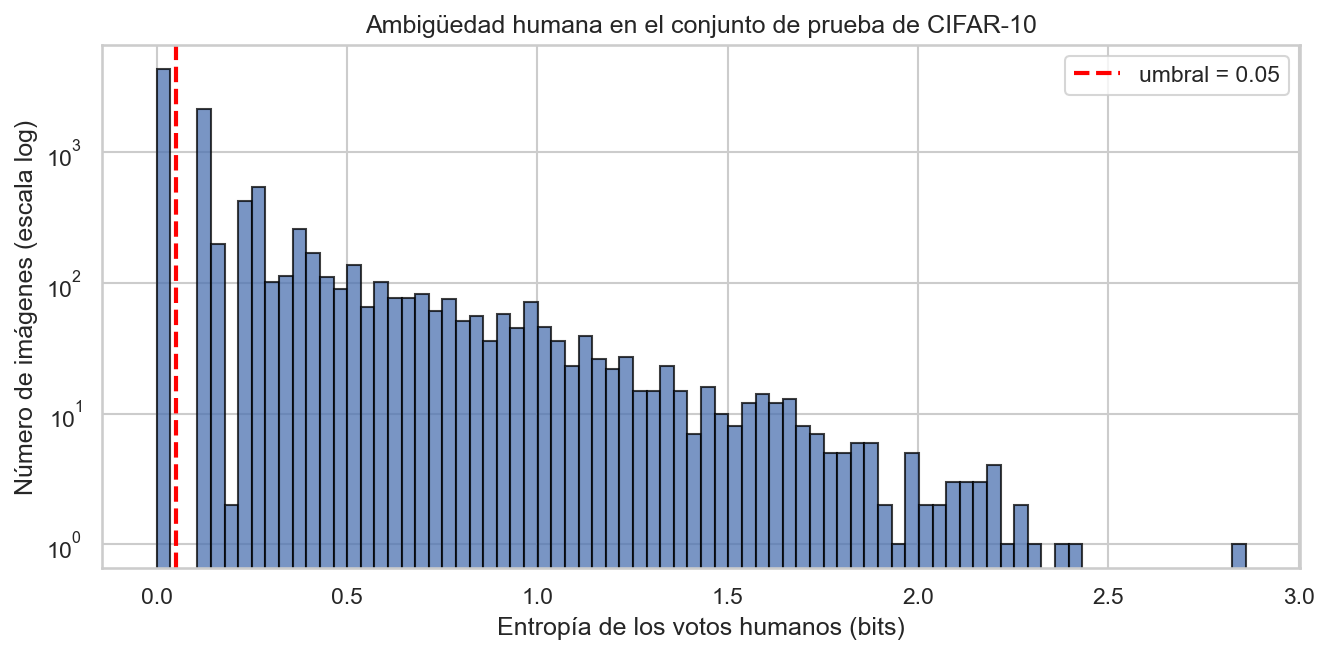
\includegraphics[width=0.9\textwidth]{fig12_h3_ambiguedad_distribucion.png}
\caption{Distribución de la entropía de los votos humanos (CIFAR-10H) sobre el
conjunto de prueba, con el umbral que separa imágenes de consenso unánime de
imágenes ambiguas.}
\label{fig:h3a}
\end{figure}

\begin{figure}[H]
\centering
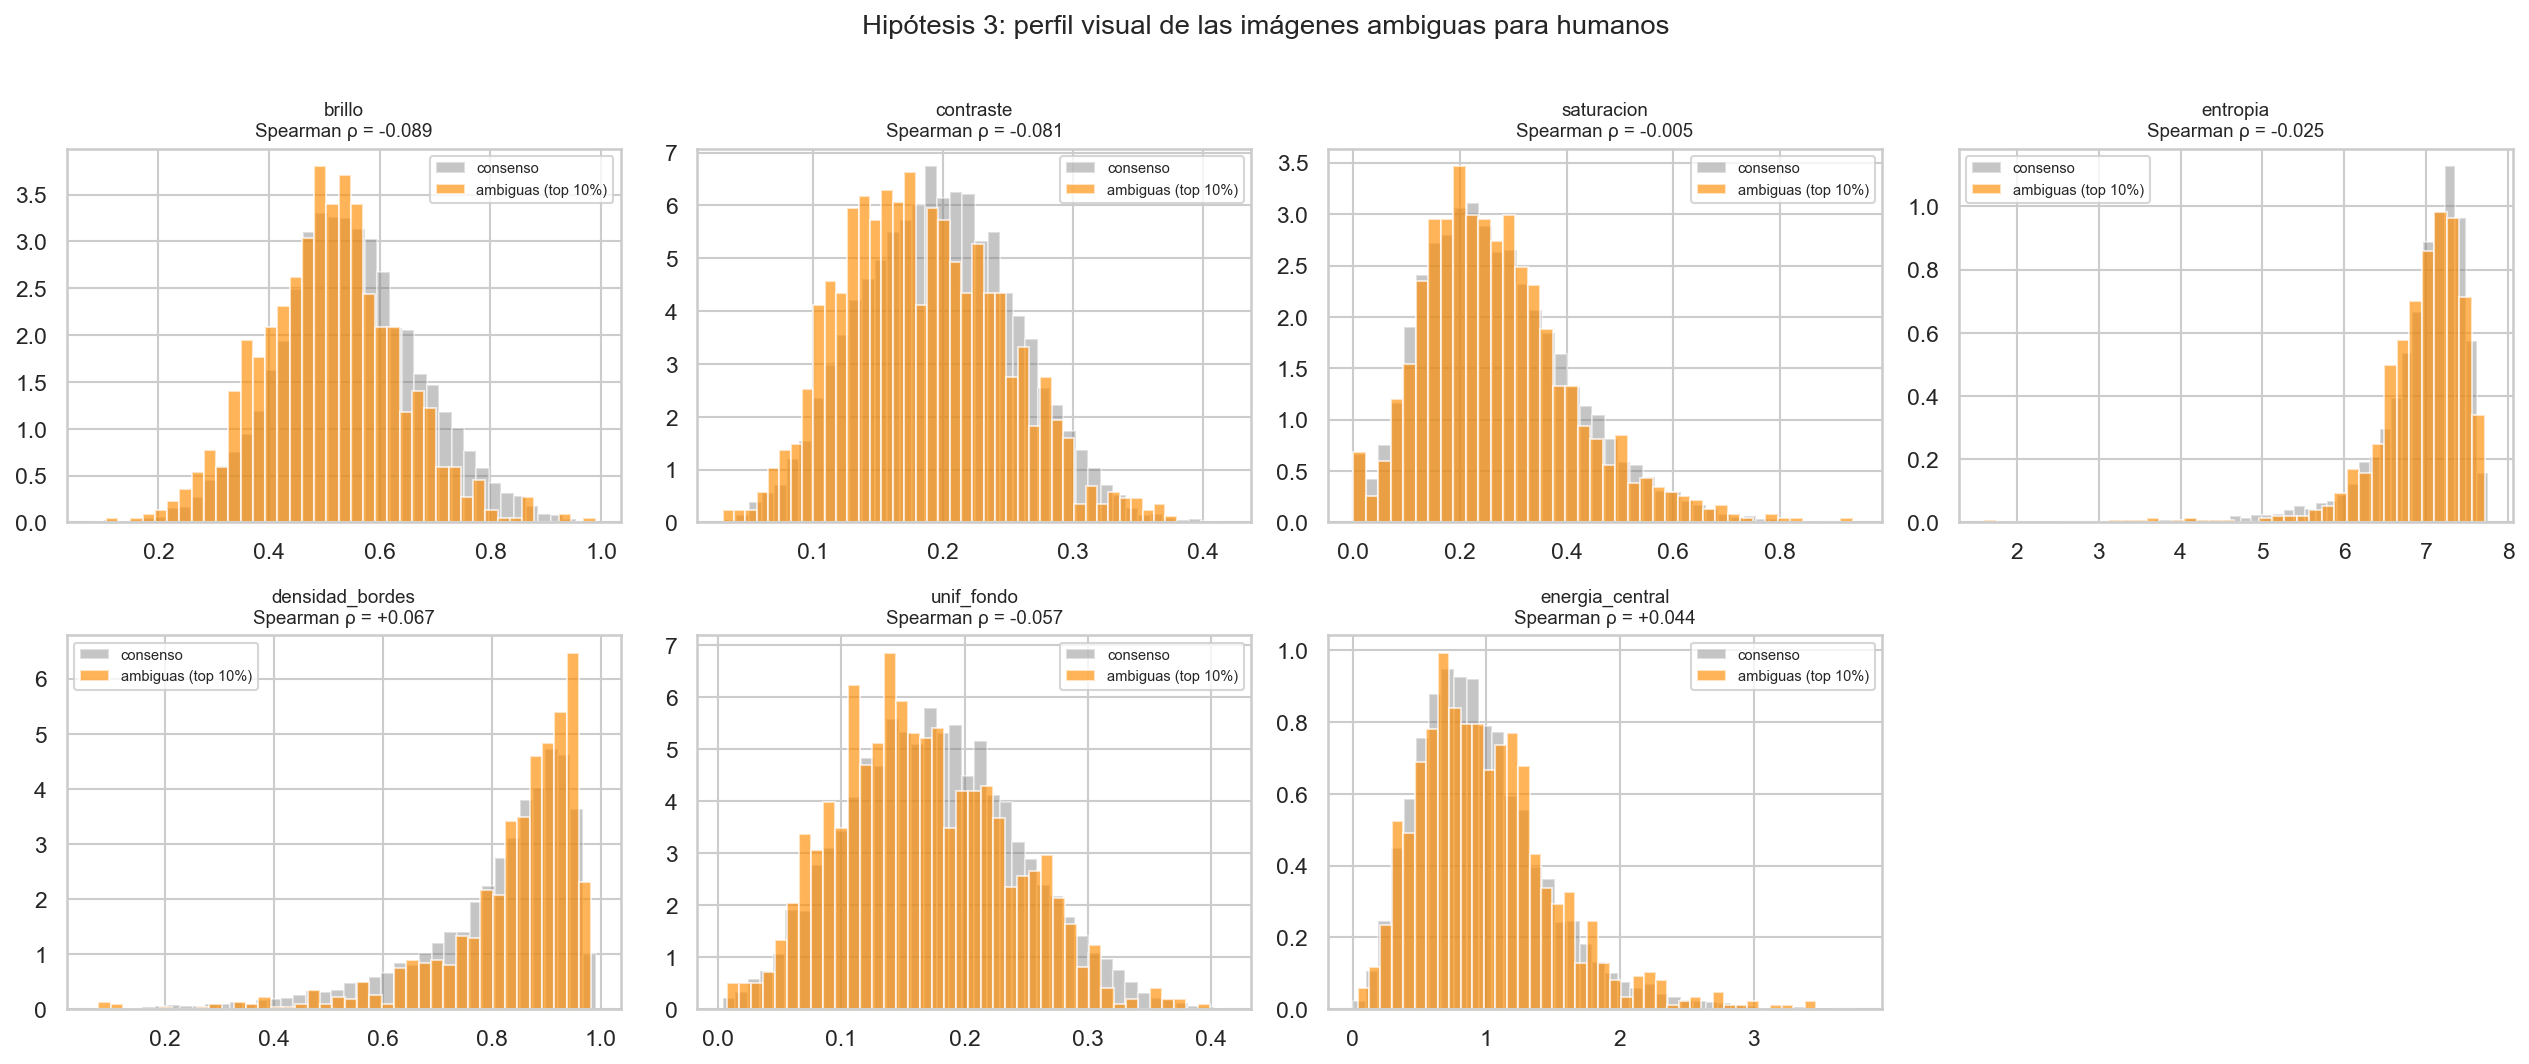
\includegraphics[width=\textwidth]{fig13_h3_ambiguedad_vs_caracteristicas.png}
\caption{Comparación del perfil de características visuales entre imágenes de
consenso unánime y imágenes de alta ambigüedad humana, y distribución de la
ambigüedad a través de los clusters.}
\label{fig:h3b}
\end{figure}

\emph{Descripción e interpretación.} Sobre las 10\,000 imágenes del conjunto de
prueba, la correlación de Spearman entre \texttt{entropia\_humana} y cada
característica visual resultó, en todos los casos, débil:

\begin{center}
\small
\begin{tabular}{@{}lrl@{}}
\toprule
\textbf{Característica} & \textbf{Spearman $\rho$} & \textbf{$p$-valor} \\
\midrule
brillo             & $-0.089$ & $5.6\times10^{-19}$ \\
densidad\_bordes   & $+0.067$ & $1.6\times10^{-11}$ \\
contraste          & $-0.081$ & $4.4\times10^{-16}$ \\
unif\_fondo        & $-0.057$ & $1.1\times10^{-8}$ \\
energia\_central   & $+0.044$ & $8.8\times10^{-6}$ \\
entropia           & $-0.025$ & $1.3\times10^{-2}$ \\
saturacion         & $-0.005$ & $0.614$ (no significativo) \\
\bottomrule
\end{tabular}
\end{center}

Con $n=10\,000$, incluso correlaciones de magnitud trivial ($|\rho|<0.1$)
resultan estadísticamente significativas; esto es un ejemplo directo de la
distinción --- vista en el Aula 03 con el cuarteto de Anscombe --- entre
significancia estadística y relevancia práctica. La característica con mayor
asociación es \texttt{brillo} ($\rho=-0.089$): imágenes ligeramente más oscuras
tienden a generar algo más de desacuerdo entre anotadores humanos, pero el
efecto es demasiado pequeño para ser explicativo por sí solo.
\texttt{saturacion} no muestra relación alguna ($p=0.614$).

\paragraph{Conclusión intermedia H3.} \textbf{No se confirma.} Las
características visuales de bajo nivel usadas en este trabajo no explican de
forma sustancial la ambigüedad percibida por humanos: todas las correlaciones
de Spearman están por debajo de $|\rho|=0.09$. La ambigüedad humana en
CIFAR-10 parece depender de factores que estas ocho variables no capturan ---
plausiblemente de naturaleza semántica (p.\,ej.\ confusión entre \emph{cat} y
\emph{dog}, o entre \emph{automobile} y \emph{truck}) antes que perceptual de
bajo nivel. Este resultado, aunque negativo, es informativo: descarta una
hipótesis razonable y redirige la pregunta hacia una comparación a nivel de
\emph{clase confundida} más que de píxel, que queda como línea futura.

\subsection{Panel resumen}

\begin{figure}[H]
\centering
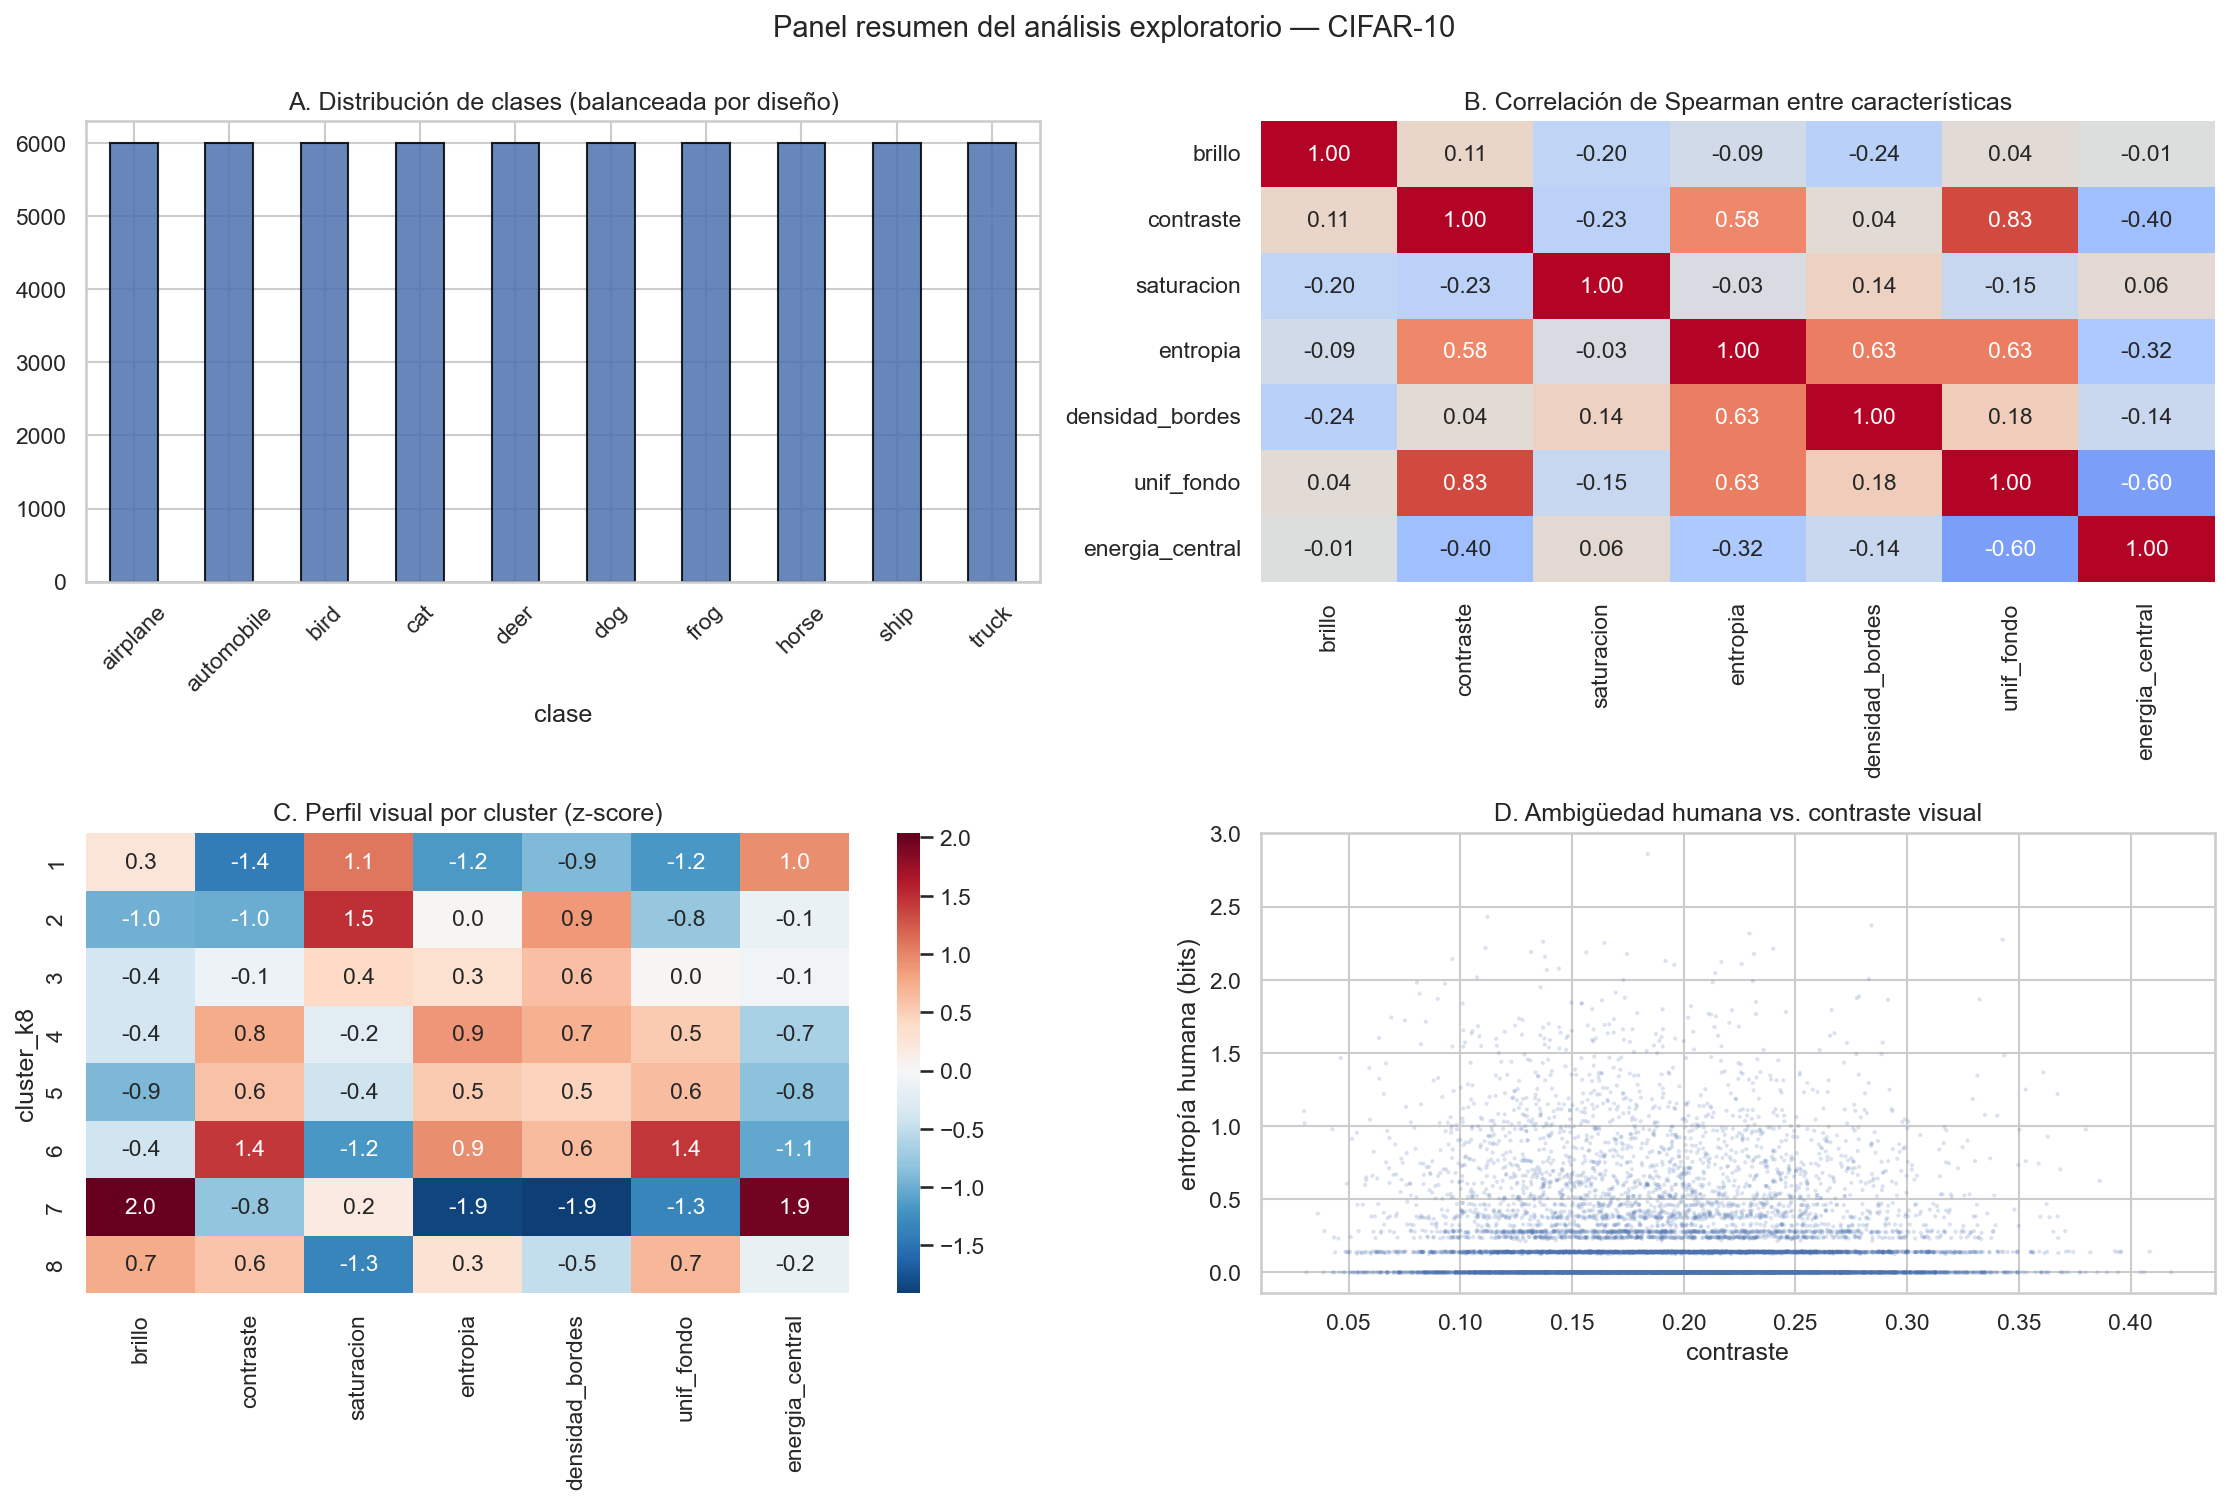
\includegraphics[width=\textwidth]{fig14_dashboard_resumen.png}
\caption{Panel integrado construido con matplotlib/seaborn: distribución de
clases, matriz de correlación, perfil de clusters y relación entre ambigüedad
humana y características visuales, en una sola vista.}
\label{fig:dashboard}
\end{figure}

%=====================  9. CONCLUSIONES  =============================
\section{Conclusiones}

\subsection{Resumen del conocimiento obtenido}

CIFAR-10 carece de atributos nativos más allá de la etiqueta de clase, pero al
dotarlo de ocho características visuales interpretables emergen dos estructuras
que la clase semántica por sí sola no revela: primero, existen agrupamientos
jerárquicos que reúnen imágenes de clases distintas cuando comparten
complejidad de fondo y textura (H1); segundo, al menos una clase (\emph{bird})
se fragmenta internamente en subgrupos visualmente diferenciados que la
etiqueta única oculta (H2). En cambio, la ambigüedad que perciben los
anotadores humanos --- medida de forma independiente en CIFAR-10H --- no se
explica por estas características de bajo nivel (H3), lo que sugiere que la
confusión humana opera a un nivel semántico que el análisis de píxeles no
alcanza a capturar. El dataset resultó además de alta calidad técnica: sin
duplicados exactos ni imágenes degeneradas, con un 10.01\,\% de registros
marcados como atípicos en al menos una característica.

\subsection{Respuesta final a cada hipótesis}

\begin{itemize}[leftmargin=*]
  \item \textbf{H1 --- Confluencia visual entre clases: se confirma.} Tres de
  ocho clusters ($k=8$) tienen pureza $<0.6$ y se distinguen del resto del
  dataset por mayor \texttt{unif\_fondo}, \texttt{densidad\_bordes} y
  \texttt{entropia} (tamaños de efecto $d\approx0.4$--$0.5$).
  \item \textbf{H2 --- Divergencia visual dentro de una clase: se confirma.}
  \emph{bird} es la clase más fragmentada ($k=18$), con subgrupos visualmente
  distinguibles por brillo, contraste y uniformidad de fondo.
  \item \textbf{H3 --- Ambigüedad humana y calidad visual: no se confirma.}
  Ninguna característica visual correlaciona de forma relevante con la entropía
  de los votos humanos de CIFAR-10H ($|\rho_{\text{Spearman}}|<0.09$ en los
  siete casos).
\end{itemize}

\subsection{Principales sorpresas y desafíos}

La mayor sorpresa fue negativa: se esperaba encontrar duplicados o
casi-duplicados dada la recolección automática de CIFAR desde buscadores web,
pero la búsqueda por \emph{hash} exacto no encontró ninguno, es un recordatorio
de que ese método solo detecta copias bit-idénticas, no recortes o
recompresiones de un mismo origen. La segunda sorpresa fue el refuerzo de H3:
se anticipaba que imágenes de baja calidad visual (bajo contraste, alta
entropía) generarían más desacuerdo humano, y el efecto resultó, en la
práctica, inexistente. El principal desafío técnico fue de escala: el
\emph{clustering} aglomerativo es $O(n^2)$ en memoria, lo que obligó a trabajar
con una submuestra estratificada de 10\,000 imágenes para las secciones que
dependen de \emph{embeddings} y clusters (H1, H2), mientras que las
características visuales de bajo nivel sí se calcularon sobre el dataset
completo (60\,000 imágenes).

\subsection{Puente hacia Visual Analytics}
\label{sec:puente}

El análisis exploratorio determina los requisitos de la herramienta interactiva
que se desarrollará en la siguiente etapa del curso:

\begin{enumerate}[leftmargin=*]
  \item \textbf{Vista jerárquica principal.} Un \emph{treemap} zoomable derivado
  del dendrograma, siguiendo el algoritmo \emph{slice-and-dice} adaptado de
  \textsc{DendroMap}, implementado en D3.js.
  \item \textbf{Panel de características acoplado.} A diferencia de
  \textsc{DendroMap}, al seleccionar un cluster se mostrarán los histogramas de
  sus características visuales contrastados contra la distribución global. Este
  es el aporte diferencial del proyecto y se justifica por los hallazgos de H1
  y H2.
  \item \textbf{Filtrado por rango de características.} Sliders que permitan
  aislar, por ejemplo, las imágenes de bajo contraste a través de todo el
  dataset, cruzando la partición por clase y por cluster.
  \item \textbf{Codificación de la ambigüedad humana.} Resaltado de las imágenes
  con alto desacuerdo entre anotadores, como apoyo a la detección de posibles
  errores de etiquetado. Derivado de H3.
  \item \textbf{Vistas coordinadas.} Selección en cualquier vista (treemap,
  histograma, scatterplot) que se propague a las demás mediante \emph{brushing
  and linking}.
\end{enumerate}

Los dos comportamientos mejor sustentados por el análisis exploratorio, y por
tanto prioritarios para la exploración interactiva, son la \textbf{confluencia
visual entre clases} (H1) y la \textbf{divergencia visual dentro de una clase}
(H2). Ambos son consecuencia directa de complementar la estructura jerárquica
de \textsc{DendroMap} con atributos interpretables, y ninguno de los dos es
analizado directamente en el artículo original. La hipótesis de ambigüedad
humana (H3), al resultar refutada con la evidencia disponible, se documenta
como hallazgo negativo y se deja como pregunta abierta para una futura
comparación a nivel semántico (pares de clases confundidas) en lugar de a nivel
de píxel.

%=====================  10. REFERENCIAS  =============================
\section{Referencias}
\label{sec:refs}

\begin{thebibliography}{9}

\bibitem{bertucci2023}
D.~Bertucci, M.~M.~Hamid, Y.~Anand, A.~Ruangrotsakun, D.~Tabatabai, M.~Perez y
M.~Kahng.
\newblock DendroMap: Visual Exploration of Large-Scale Image Datasets for
Machine Learning with Treemaps.
\newblock \emph{IEEE Transactions on Visualization and Computer Graphics},
29(1):320--330, 2023. DOI: 10.1109/TVCG.2022.3209425.

\bibitem{krizhevsky2009}
A.~Krizhevsky.
\newblock Learning Multiple Layers of Features from Tiny Images.
\newblock Technical Report, University of Toronto, 2009.
\newblock \url{https://www.cs.toronto.edu/~kriz/cifar.html}

\bibitem{peterson2019}
J.~C.~Peterson, R.~M.~Battleday, T.~L.~Griffiths y O.~Russakovsky.
\newblock Human Uncertainty Makes Classification More Robust.
\newblock \emph{Proceedings of the IEEE/CVF International Conference on Computer
Vision (ICCV)}, pp.~9617--9626, 2019.

\bibitem{li2024}
Y.~Li et al.
\newblock Visual Analytics for Efficient Image Exploration and User-Guided Image
Captioning.
\newblock \emph{IEEE Transactions on Visualization and Computer Graphics},
30(6):2875--2887, 2024. DOI: 10.1109/TVCG.2024.3388514.

\bibitem{shneiderman1992}
B.~Shneiderman.
\newblock Tree Visualization with Tree-maps: 2-d Space-filling Approach.
\newblock \emph{ACM Transactions on Graphics}, 11(1):92--99, 1992.

\bibitem{maaten2008}
L.~van~der~Maaten y G.~Hinton.
\newblock Visualizing Data using t-SNE.
\newblock \emph{Journal of Machine Learning Research}, 9(86):2579--2605, 2008.

\bibitem{murtagh1983}
F.~Murtagh.
\newblock A Survey of Recent Advances in Hierarchical Clustering Algorithms.
\newblock \emph{The Computer Journal}, 26(4):354--359, 1983.

\bibitem{he2016}
K.~He, X.~Zhang, S.~Ren y J.~Sun.
\newblock Deep Residual Learning for Image Recognition.
\newblock \emph{IEEE Conference on Computer Vision and Pattern Recognition
(CVPR)}, pp.~770--778, 2016.

\end{thebibliography}

%=====================  11. ANEXOS  ==================================
\section{Anexos}

\subsection*{A. Notebook}

El \emph{notebook} completo, limpio y reproducible se encuentra en el
repositorio del proyecto:

\begin{center}
\url{https://github.com/DiegoRivas1/cd-visual-analytics-cifar}
\end{center}

Ruta dentro del repositorio: \texttt{notebooks/01\_eda\_cifar.ipynb}.

\subsection*{B. Reproducibilidad}

\begin{itemize}[leftmargin=*]
  \item Los archivos de datos no se versionan (superan el límite de tamaño de
  GitHub). El \emph{script} \texttt{src/download\_data.py} los descarga en
  \texttt{data/raw/}.
  \item Semilla aleatoria fijada en 42 para toda submuestra o inicialización.
  \item Entorno declarado en \texttt{requirements.txt}.
  \item Los resultados intermedios costosos (\emph{embeddings}, dendrograma) se
  cachean en \texttt{data/processed/}.
\end{itemize}

\subsection*{C. Demo de referencia}

Demo pública de \textsc{DendroMap}: \url{https://div-lab.github.io/dendromap/}\\
Código fuente: \url{https://github.com/div-lab/dendromap}

\end{document}